\documentclass{beamer}
\usetheme{Warsaw}


\iftrue

\setbeamercolor{normal text}{fg=white,bg=black!90}
\setbeamercolor{structure}{fg=white}

\setbeamercolor{alerted text}{fg=red!85!black}

\setbeamercolor{item projected}{use=item,fg=black,bg=item.fg!35}

\setbeamercolor*{palette primary}{use=structure,fg=structure.fg}
\setbeamercolor*{palette secondary}{use=structure,fg=structure.fg!95!black}
\setbeamercolor*{palette tertiary}{use=structure,fg=structure.fg!90!black}
\setbeamercolor*{palette quaternary}{use=structure,fg=structure.fg!95!black,bg=black!80}

\setbeamercolor*{framesubtitle}{fg=white}

\setbeamercolor*{block title}{parent=structure,bg=black!60}
\setbeamercolor*{block body}{fg=black,bg=black!10}
\setbeamercolor*{block title alerted}{parent=alerted text,bg=black!15}
\setbeamercolor*{block title example}{parent=example text,bg=black!15}

\fi


\begin{document}

{
    \usebackgroundtemplate
    {
        \vbox to \paperheight{\vfil\hbox to \paperwidth{\hfil

        {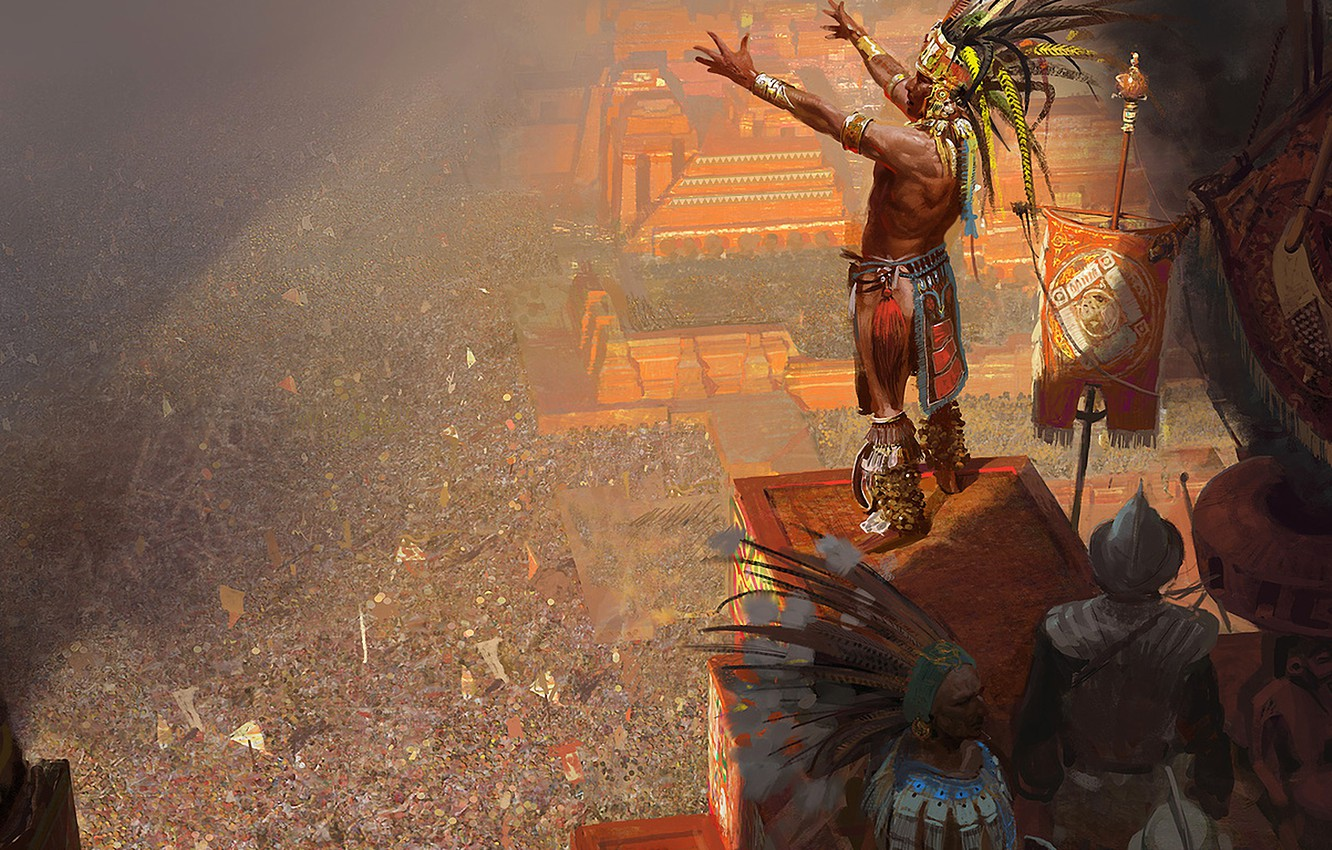
\includegraphics[width=5.05in]{../images/aztec.jpg}}

        \hfil}\vfil}
    }

    \begin{frame}
     \centering
     {
        \begin{minipage}{18cm}
           {\LARGE \color{white}{\bf reinforcement learning}} \\
           {\LARGE \color{white}{\bf with self supervised learning}} \\
           {\LARGE \color{white}{\bf - Conquista of Montezuma's Revenge}} \\
           {\LARGE \color{white}{\bf Michal CHOVANEC, PhD.}} \\
       \end{minipage}
     }

    \end{frame}
}


\begin{frame}
  \frametitle{net of doom - doom playing model}
  
    \centering
    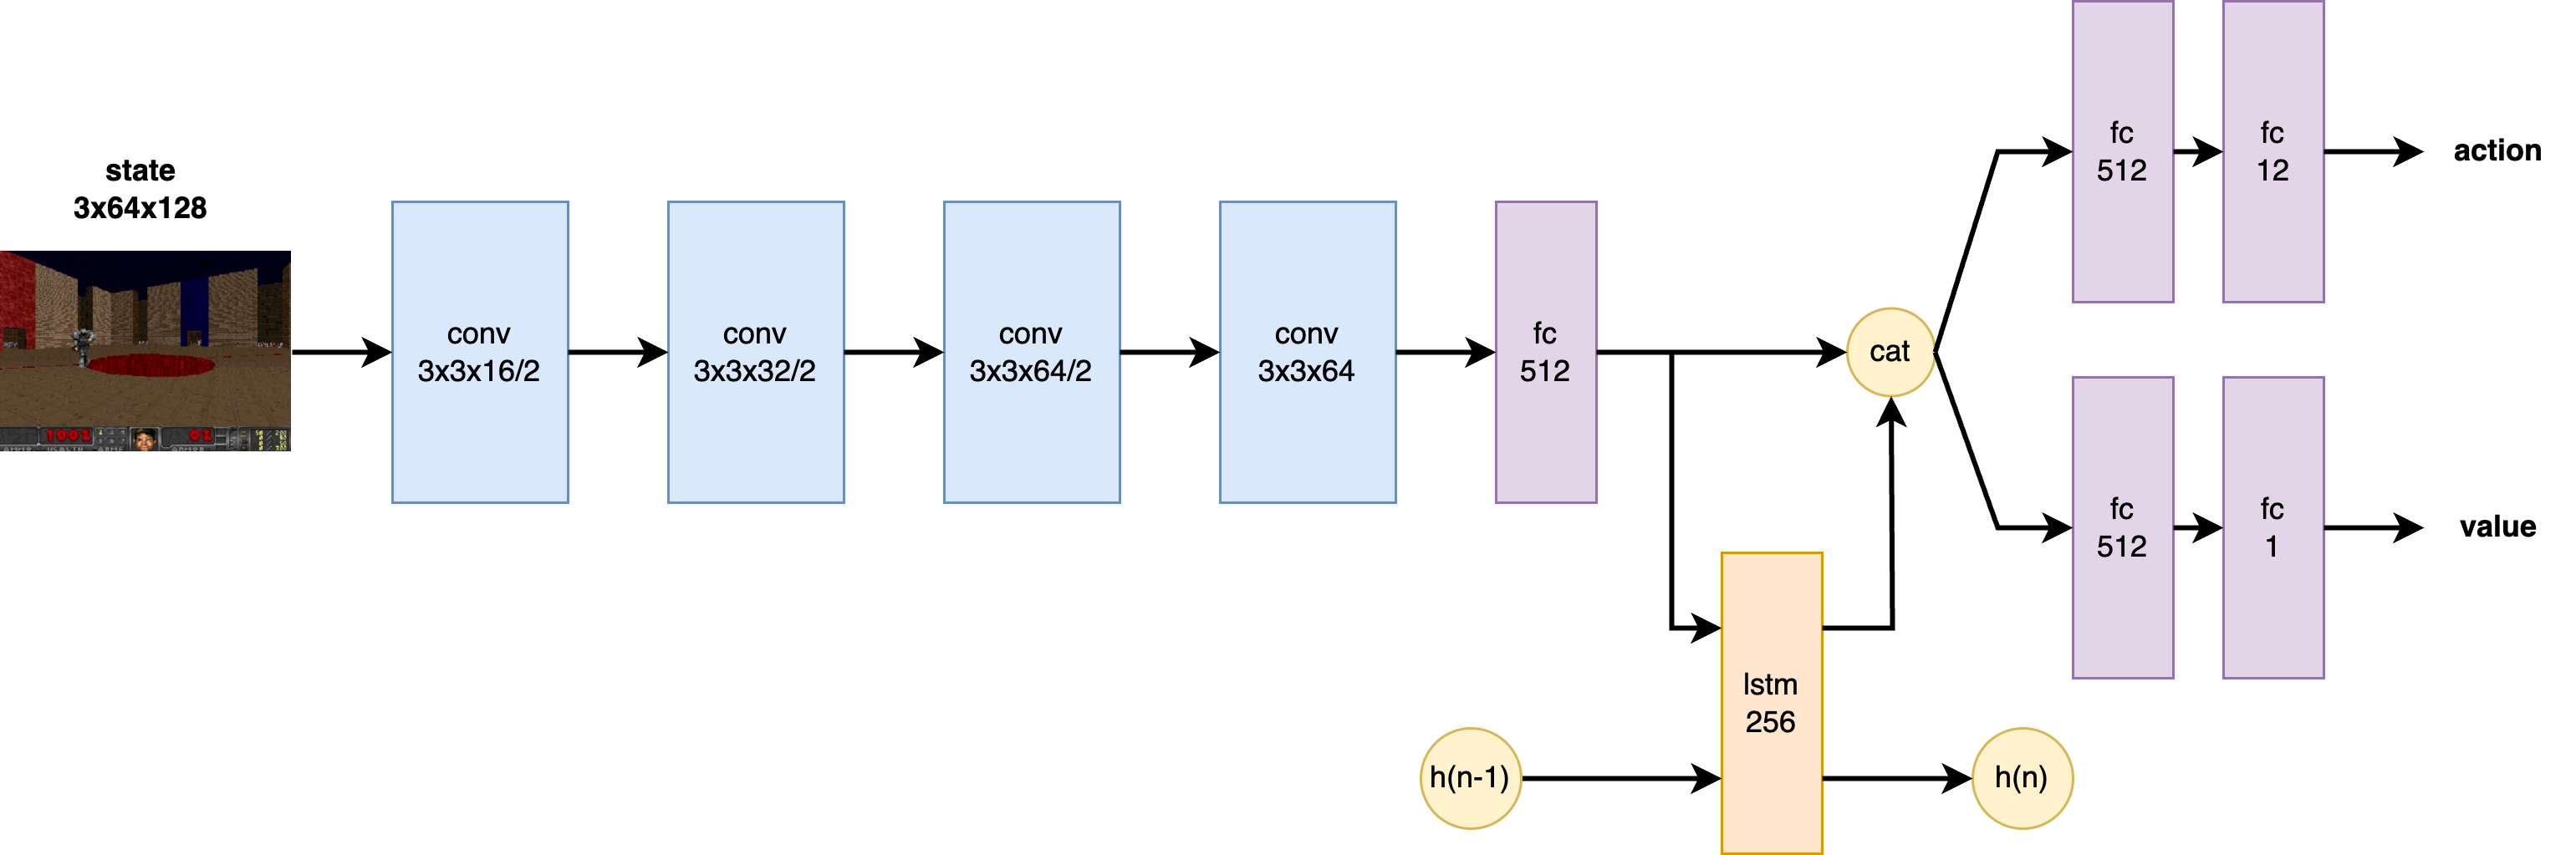
\includegraphics[scale=0.45]{../diagrams/rl_models/net_of_doom.png}
    
\end{frame}

\begin{frame}
\frametitle{reinforcement learning}
  
  \begin{columns}
  
    \begin{column}{0.5\textwidth}
      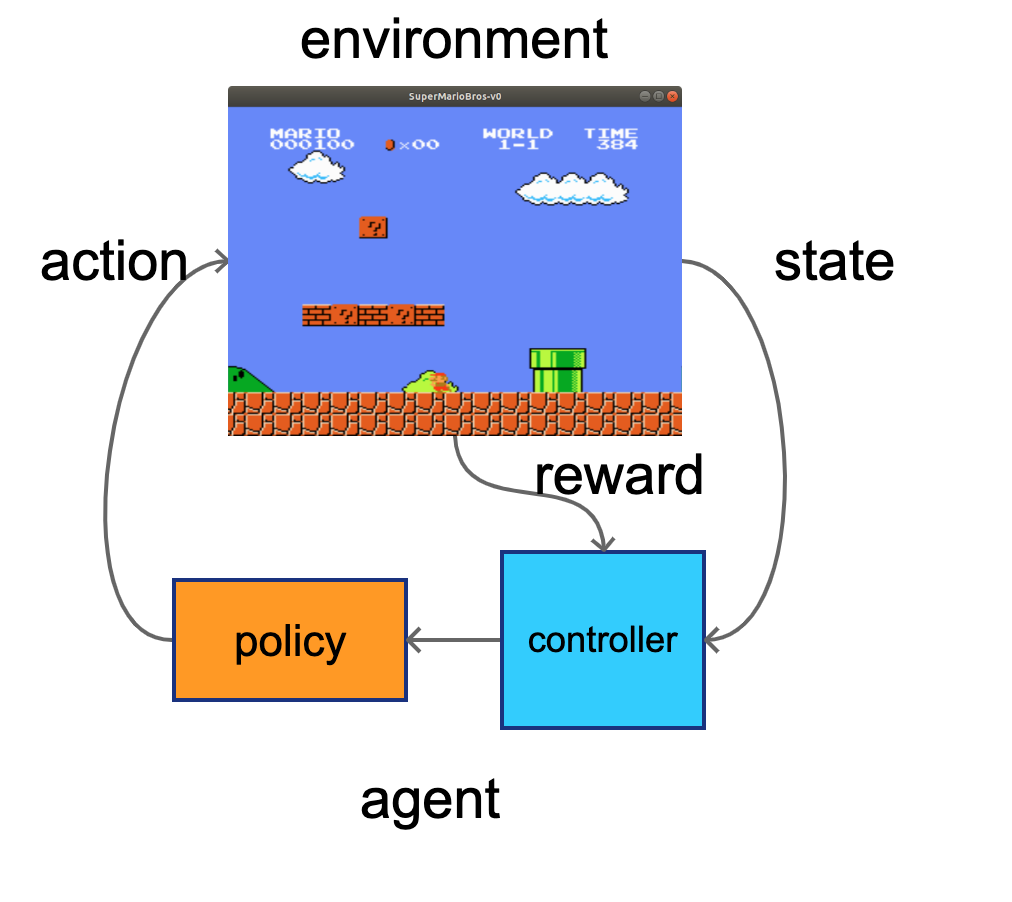
\includegraphics[scale=0.15]{../diagrams/basic/reinforcementlearning.png}
    \end{column}
  
    \begin{column}{0.5\textwidth}
      \begin{enumerate}
        \item {\bf obtain state} - observation
        \item {\bf choose action} - policy
        \item {\bf receive reward}
        \item {\bf learn from experiences}
      \end{enumerate}
    \end{column}
  
  \end{columns}
  
\end{frame}



\begin{frame}
  \frametitle{reinforcement learning - success story}
  
  \href{https://www.nature.com/articles/nature16961}{Mastering the game of Go with deep neural networks and tree search, Nature, 2016}
  \centering
  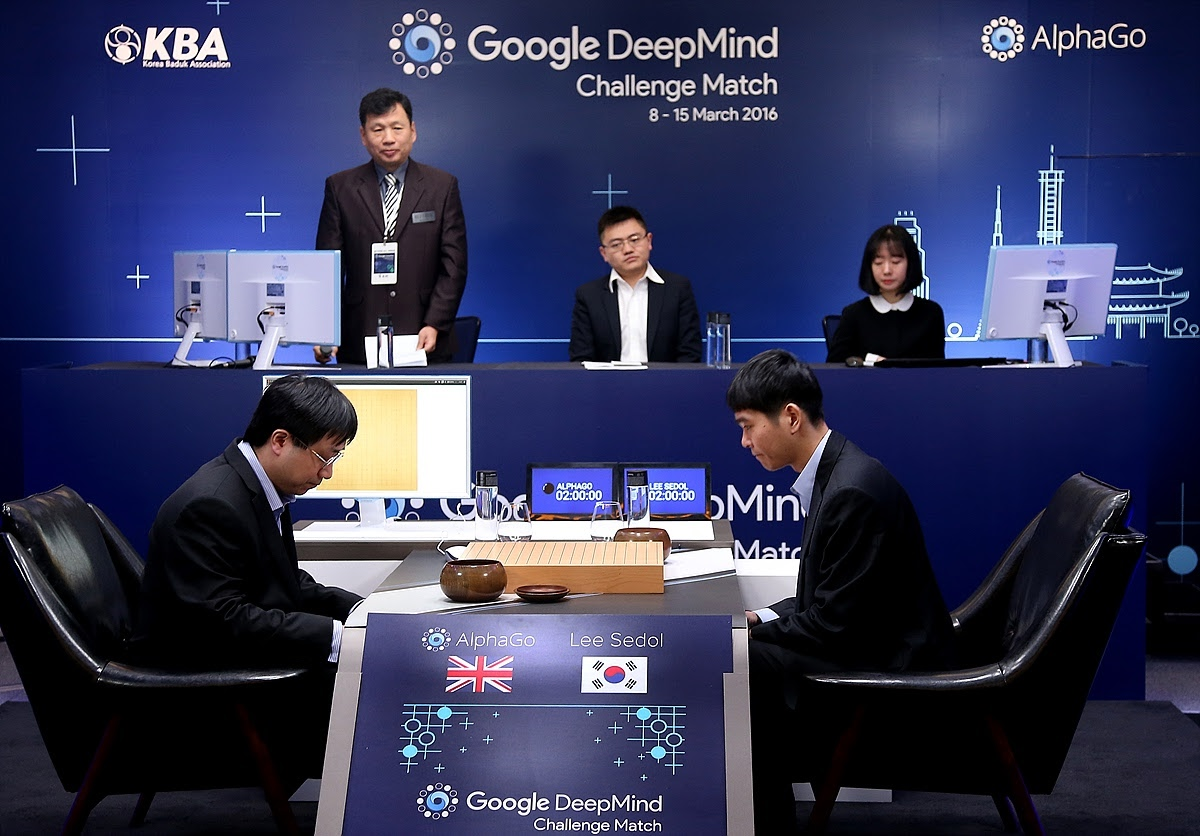
\includegraphics[scale=0.25]{../images/alpha_go.jpg}
    
\end{frame}


\begin{frame}
  \frametitle{reinforcement learning - success story}
  
  \href{https://arxiv.org/abs/2107.04034}{RMA: Rapid Motor Adaptation for Legged Robots}
  \centering
  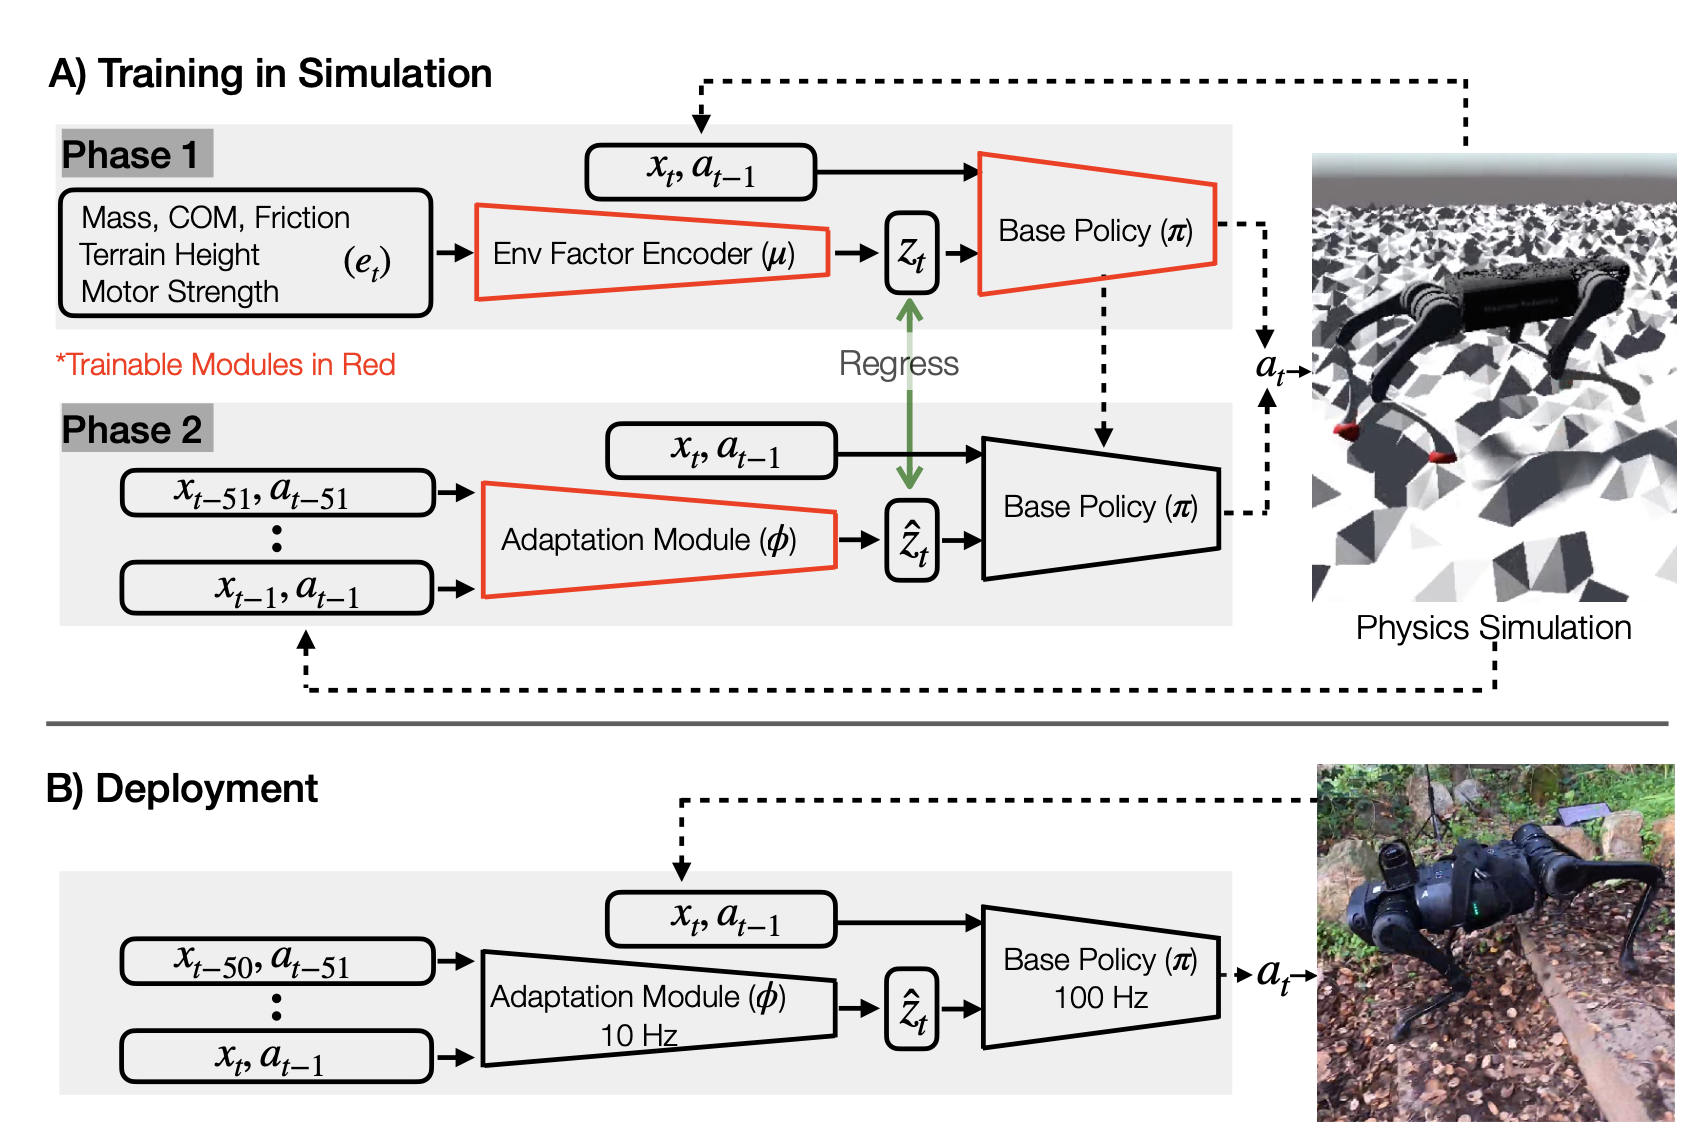
\includegraphics[scale=0.35]{../images/rma.png}
    
\end{frame}


\begin{frame}
  \frametitle{reinforcement learning - success story}
  
  \href{https://www.nature.com/articles/s41586-023-06419-4}{Champion-level drone racing using deep reinforcement learning, 2021}
  \centering
  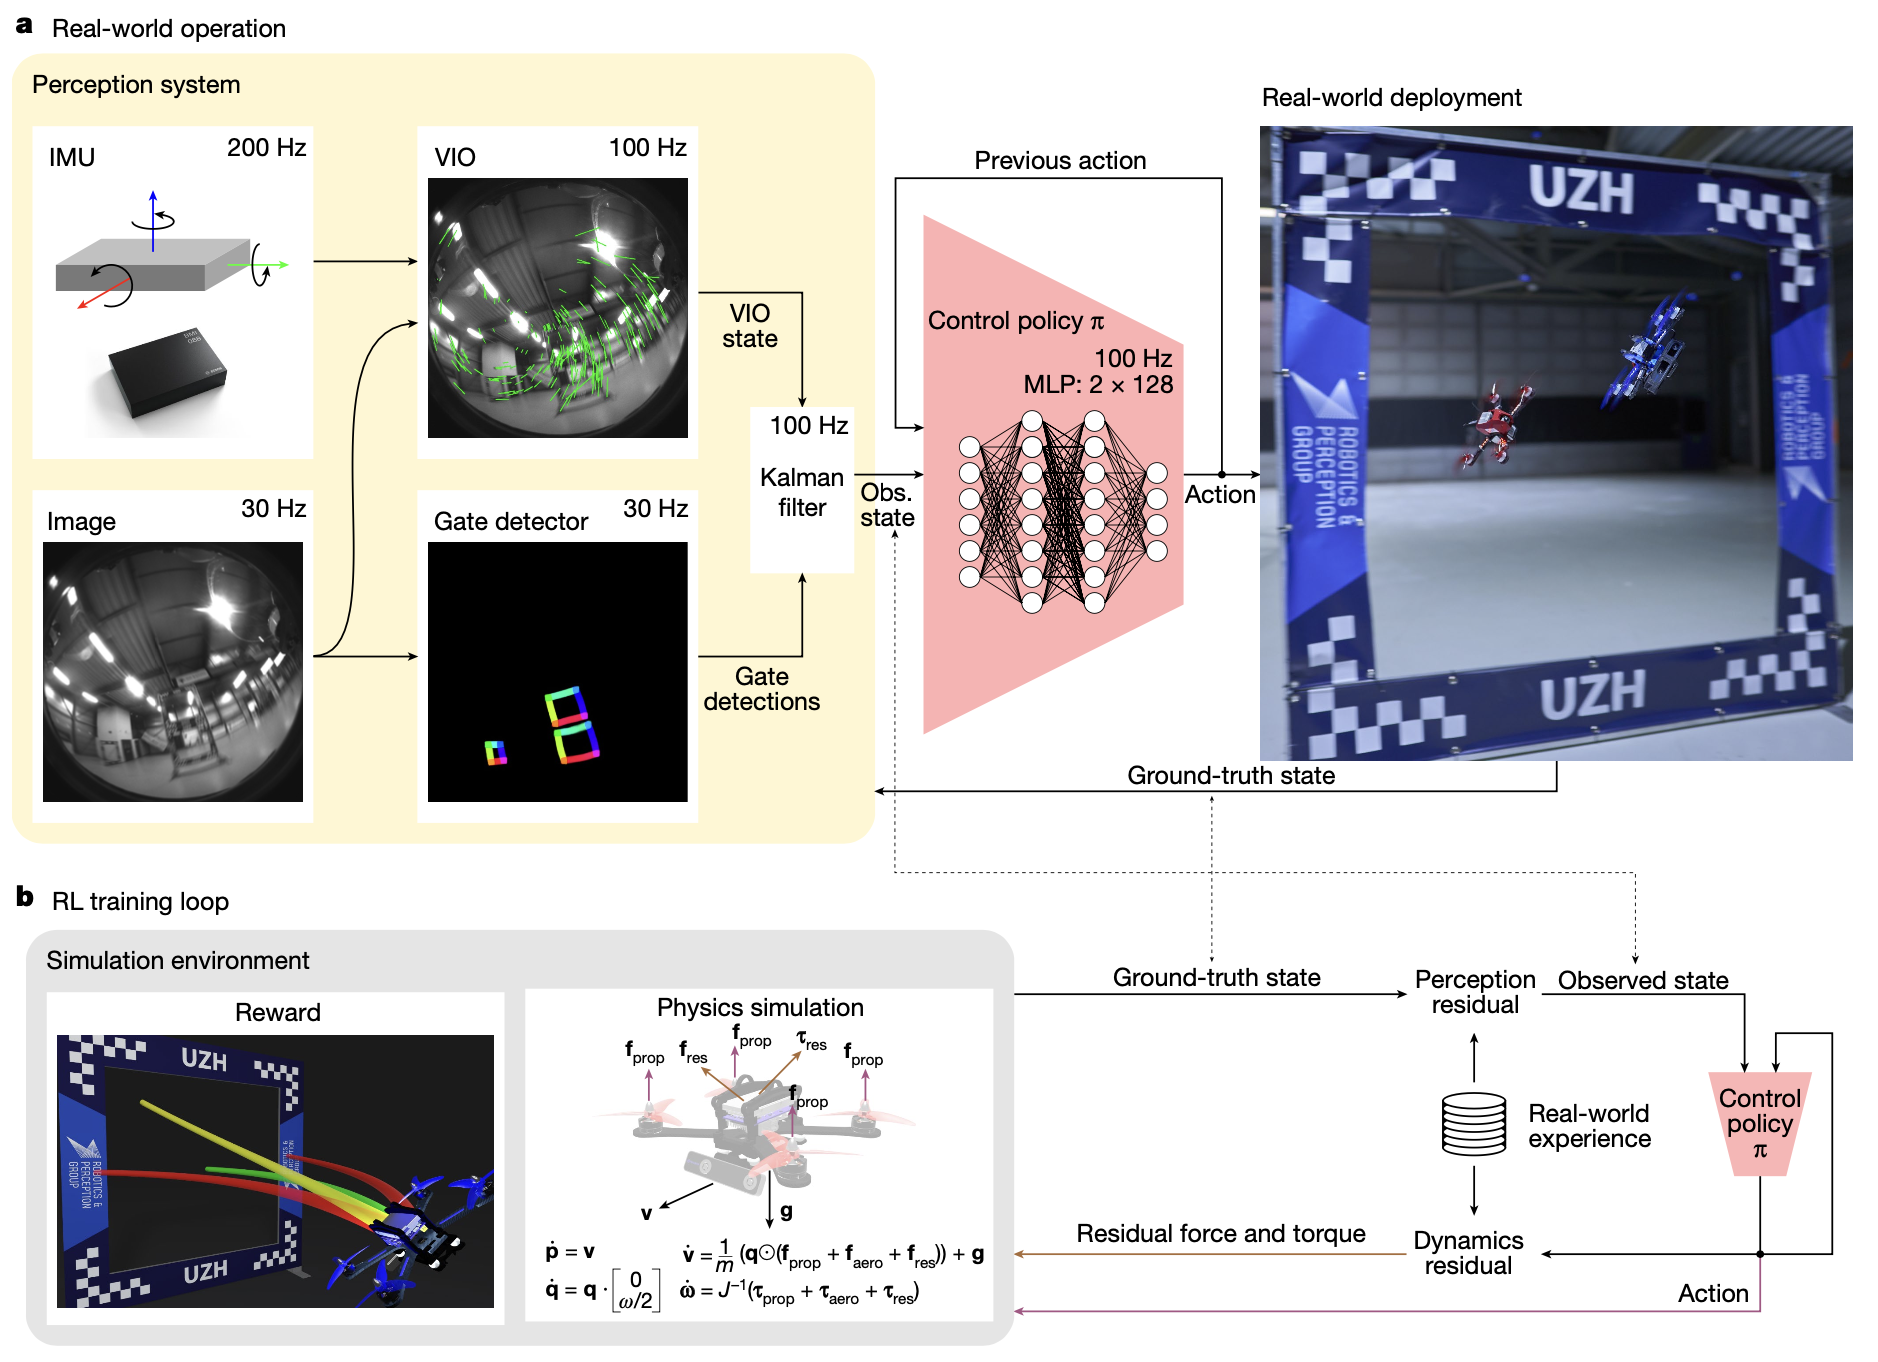
\includegraphics[scale=0.3]{../images/rl_drone.png}
    
\end{frame}


\begin{frame}
  \frametitle{reinforcement learning - success story}
  Motoko line following robot \\
  \centering
  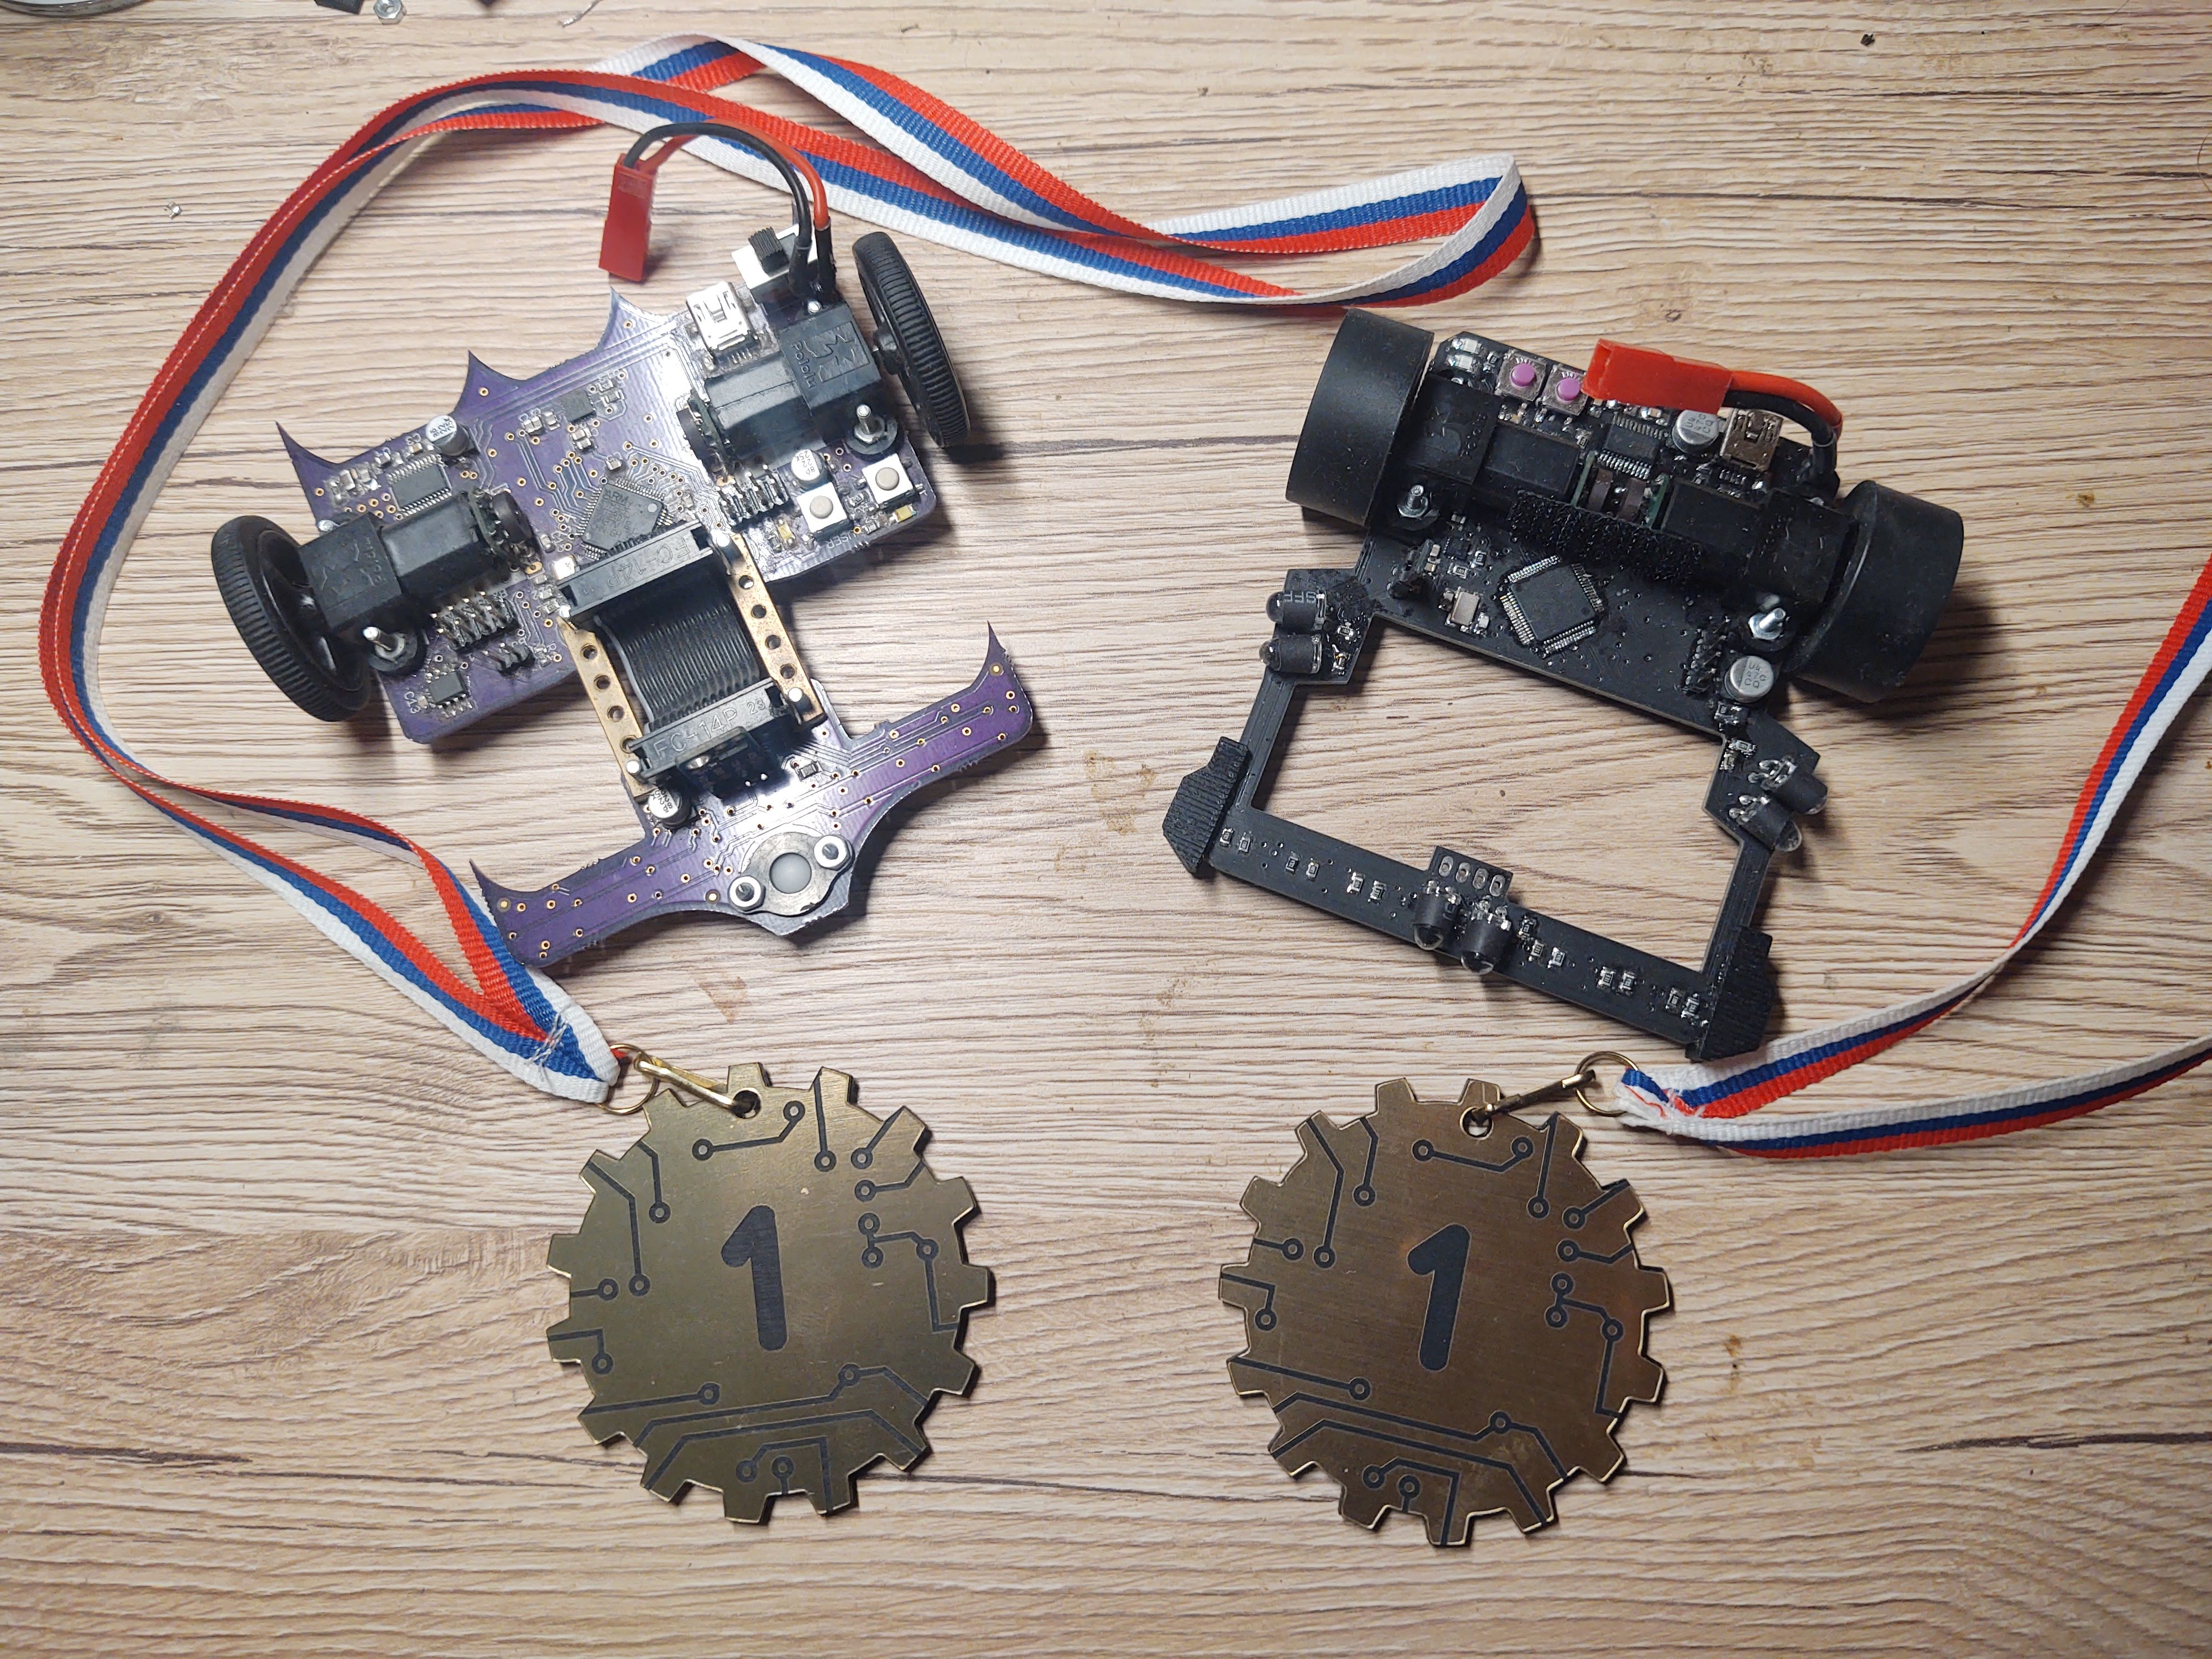
\includegraphics[scale=0.07]{../images/medals.jpg}
    
\end{frame}


\begin{frame}
  \frametitle{reinforcement learning - success story}
  Stockfish NNUE Chess engine \\
  \centering
  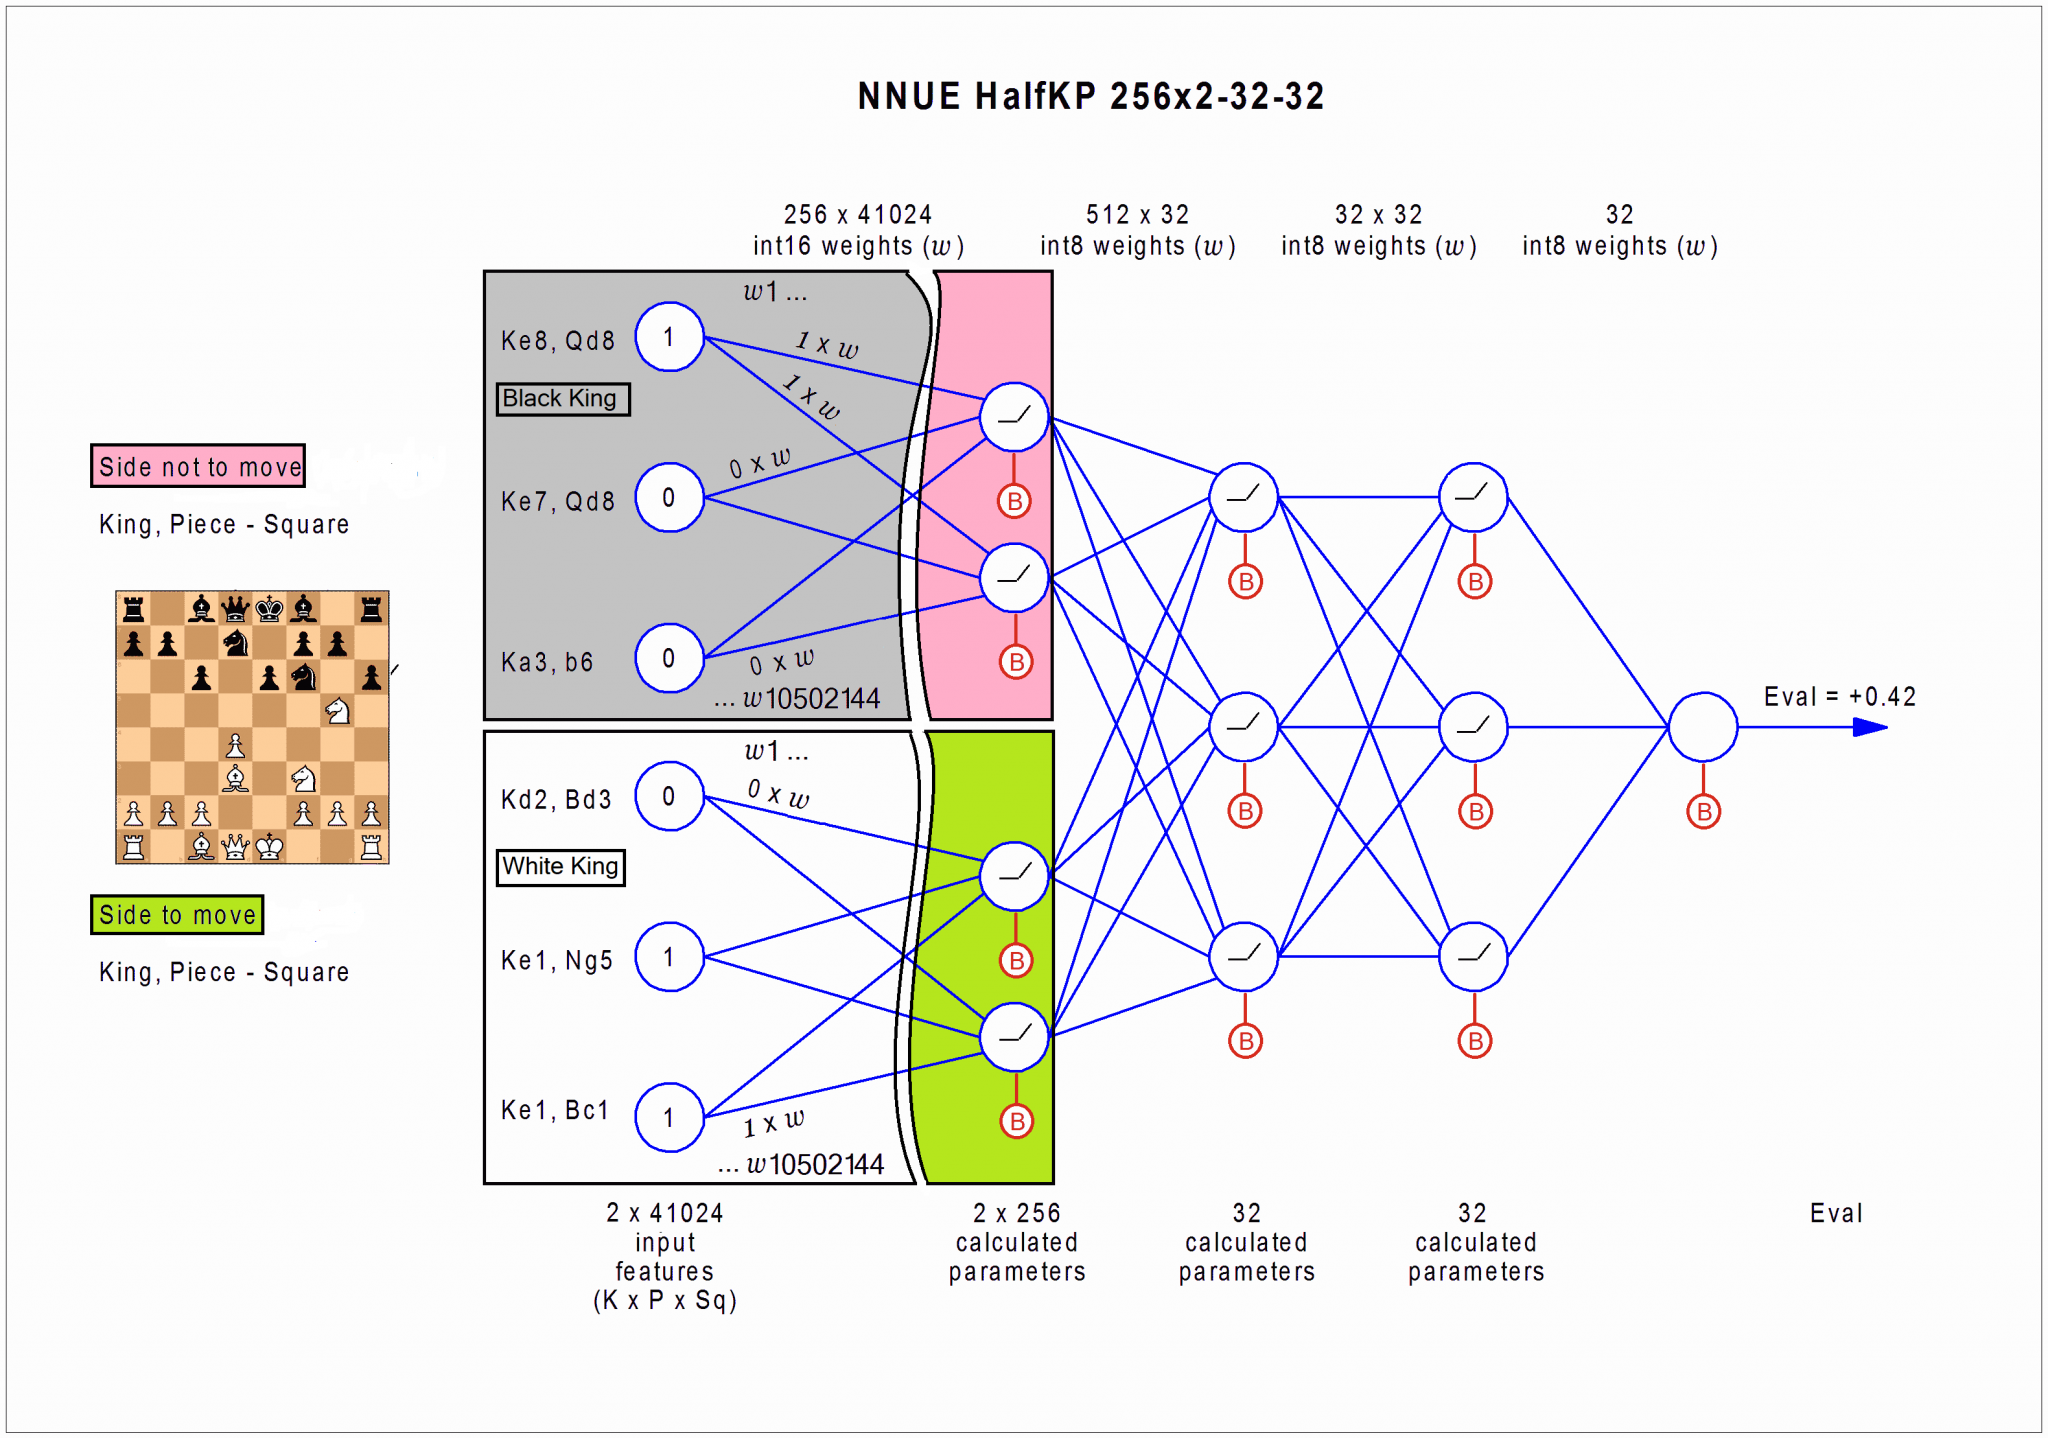
\includegraphics[scale=0.18]{../images/nnue.png}
    
\end{frame}


\begin{frame}
\frametitle{self supervised learning}

  \centering
  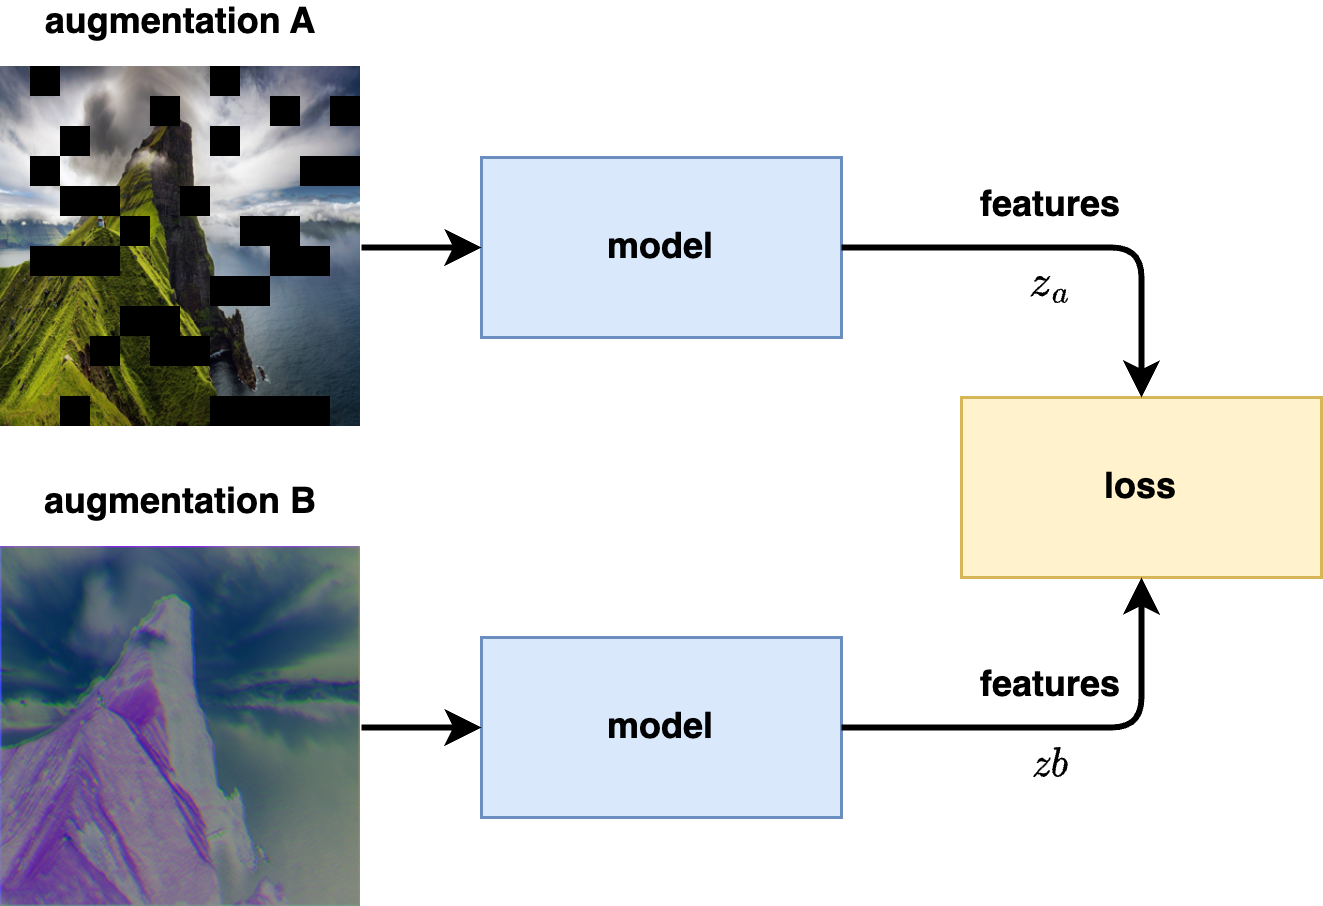
\includegraphics[scale=0.8]{../diagrams/self_supervised/self_supervised-basic.png}

  \begin{align*}
    \mathcal{L} = \vert z_a - z_b \vert^2_2
  \end{align*}

\end{frame}


\begin{frame}
\frametitle{self supervised learning - loss collapse}
  
    \centering
    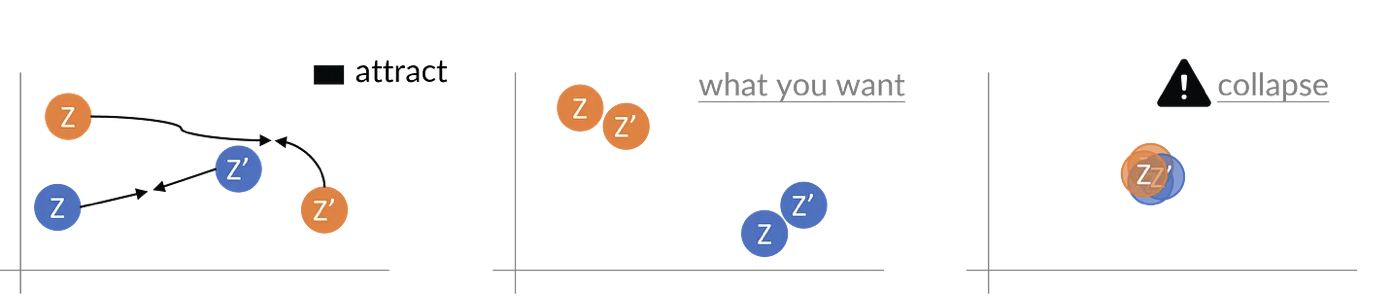
\includegraphics[scale=0.45]{../images/contrastive_loss.png}
  
\end{frame}



\begin{frame}
\frametitle{self supervised learning - contrastive loss}
  
    \centering
    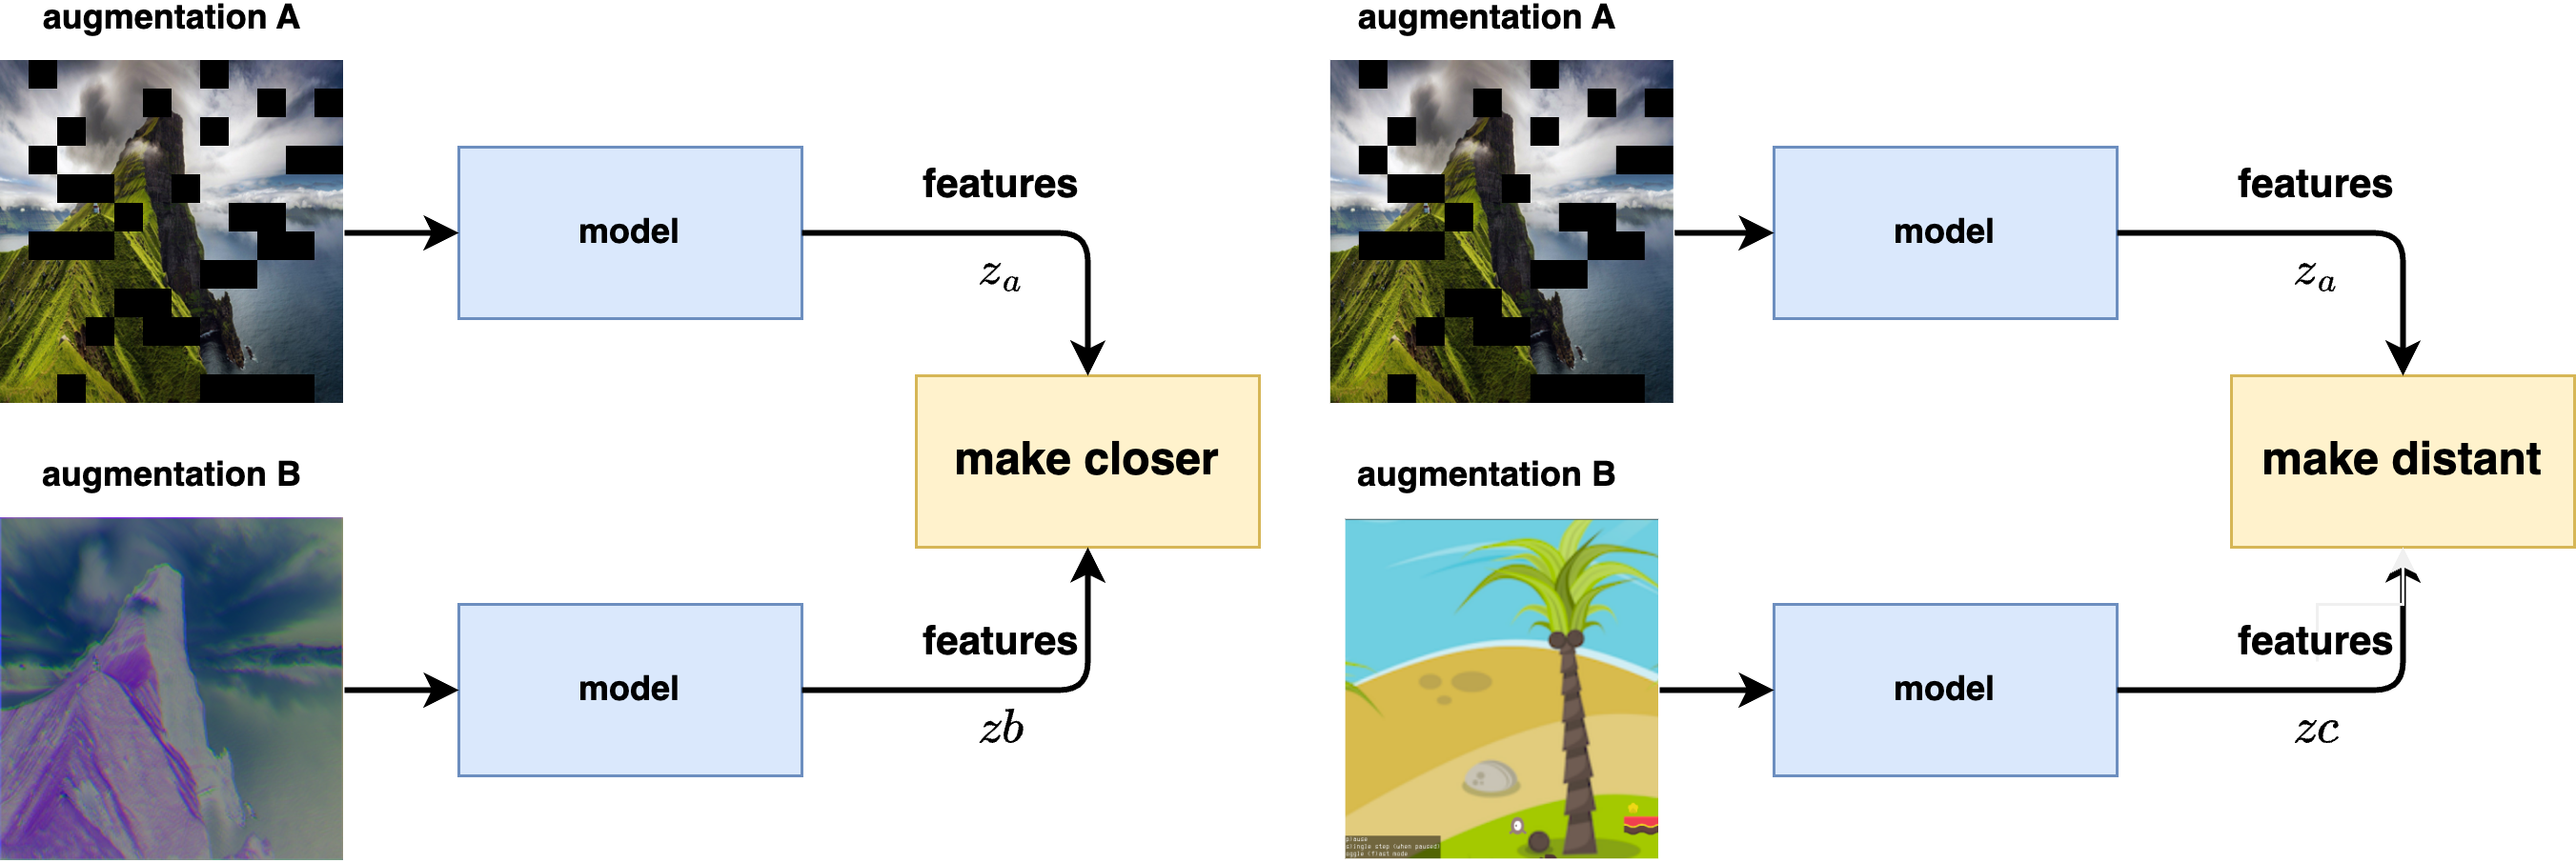
\includegraphics[scale=0.5]{../diagrams/self_supervised/self_supervised-contrastive.png}

    \begin{align*}
      \mathcal{L} = \vert z_a - z_b \vert^2_2 - \vert z_a - z_c \vert^2_2
    \end{align*}

\end{frame}



\begin{frame}
  \frametitle{VICReg - non contrastive supervised learning}

    \begin{itemize}
      \item \href{https://arxiv.org/abs/2105.04906}{VICReg: Variance-Invariance-Covariance Regularization for Self-Supervised Learning} 
      \item \href{https://www.youtube.com/watch?v=SGzMElJ11Cc}{Yann LeCun: Dark Matter of Intelligence and Self-Supervised Learning} 
    \end{itemize}
    
    \centering
    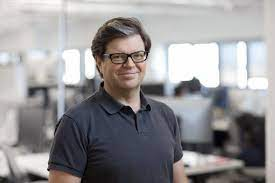
\includegraphics[scale=0.5]{../images/prof_yann_lecun.jpg}

\end{frame}



\begin{frame}
  \frametitle{VICReg - non contrastive self supervised learning}

    \begin{itemize}
      \item VAriance    $$\mathcal{L}_{variance}   = \frac{1}{N} \sum_n \max(0, 1 - std(z^*_{n, :})) $$
      \item INvariance  $$\mathcal{L}_{invariance} = \frac{1}{N} \sum_n \vert z^a_{n,:} - z^b_{n,:} \vert^2_2 $$
      \item Covariance  $$\mathcal{L}_{covariance} = \frac{1}{F} \sum_{i \neq j} cov(z^*_{:, i}, z^*_{:, j}) $$
    \end{itemize}
     
\end{frame}



\begin{frame}
  \frametitle{another loss examples}

  \centering
  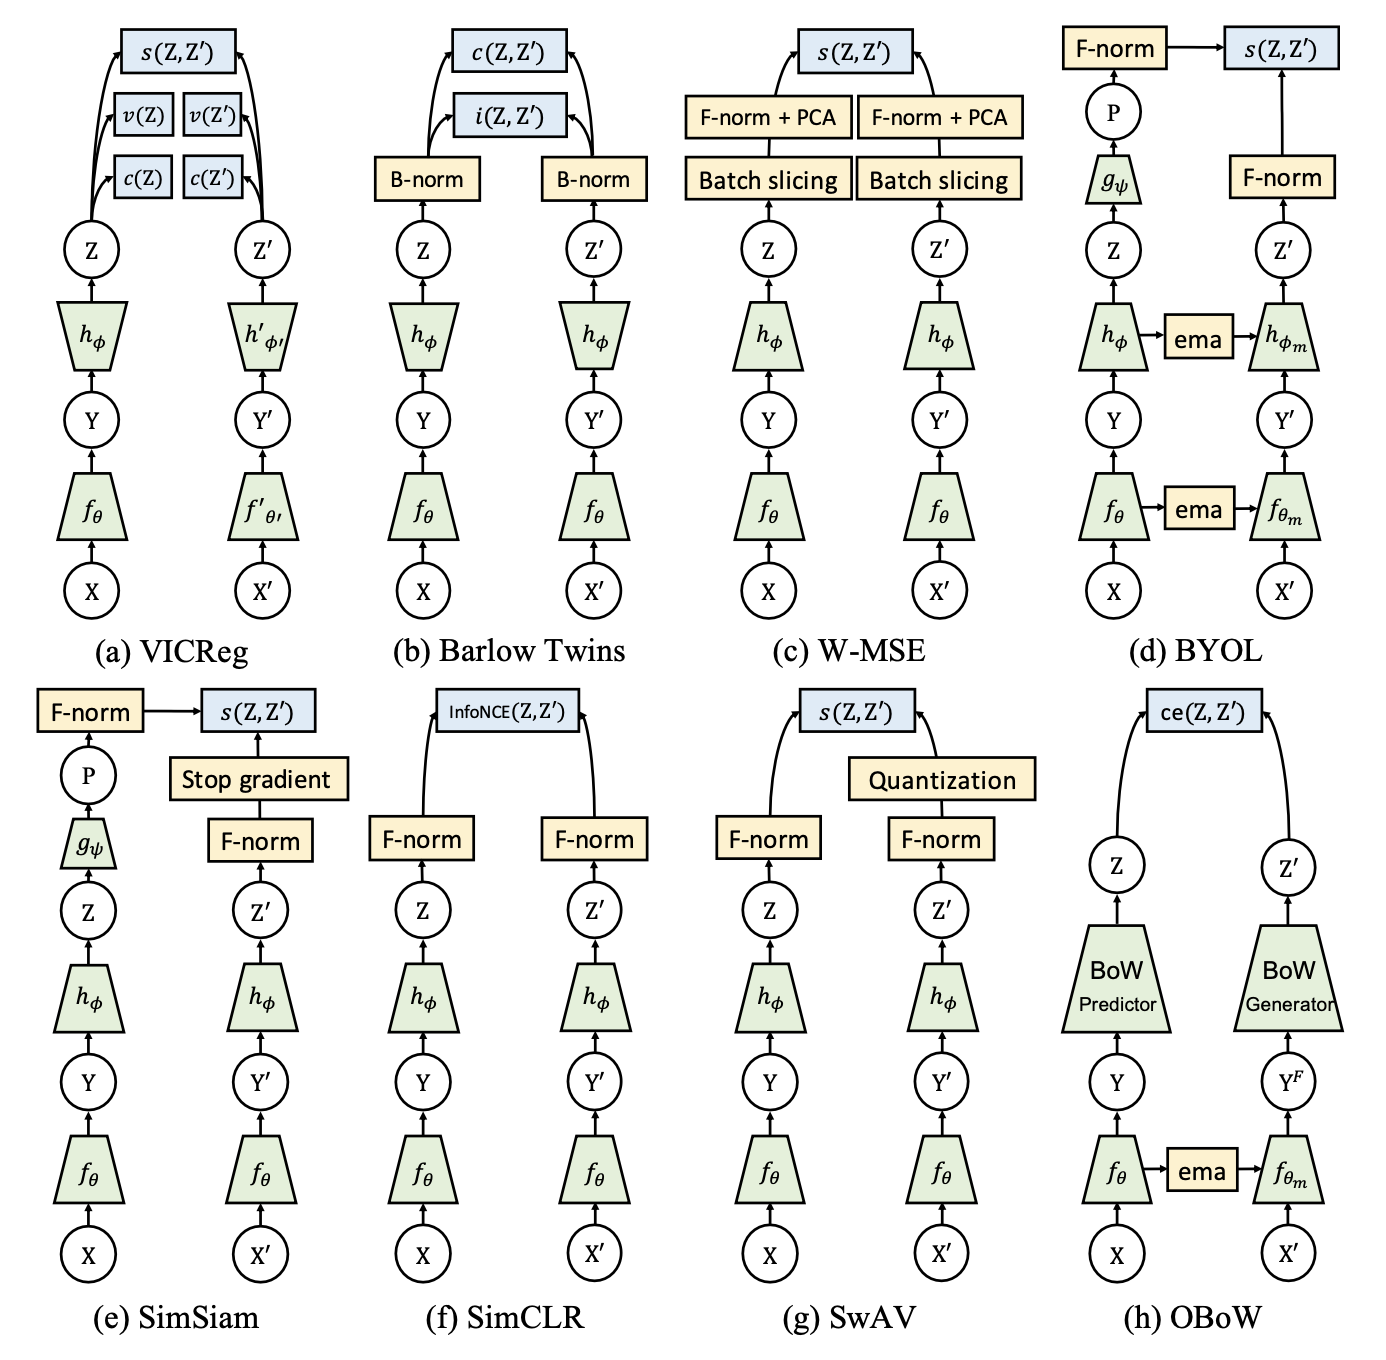
\includegraphics[scale=0.3]{../images/self_supervised_loss.png}
     
\end{frame}



\begin{frame}
  \frametitle{applications}

  \begin{itemize}
    \item face, signature matching
    \item anomaly detection
    \item e-shop similar goods finding
    \item searching by image - Google lens
    \item less labeled data for self supervised training
  \end{itemize}

  \centering
  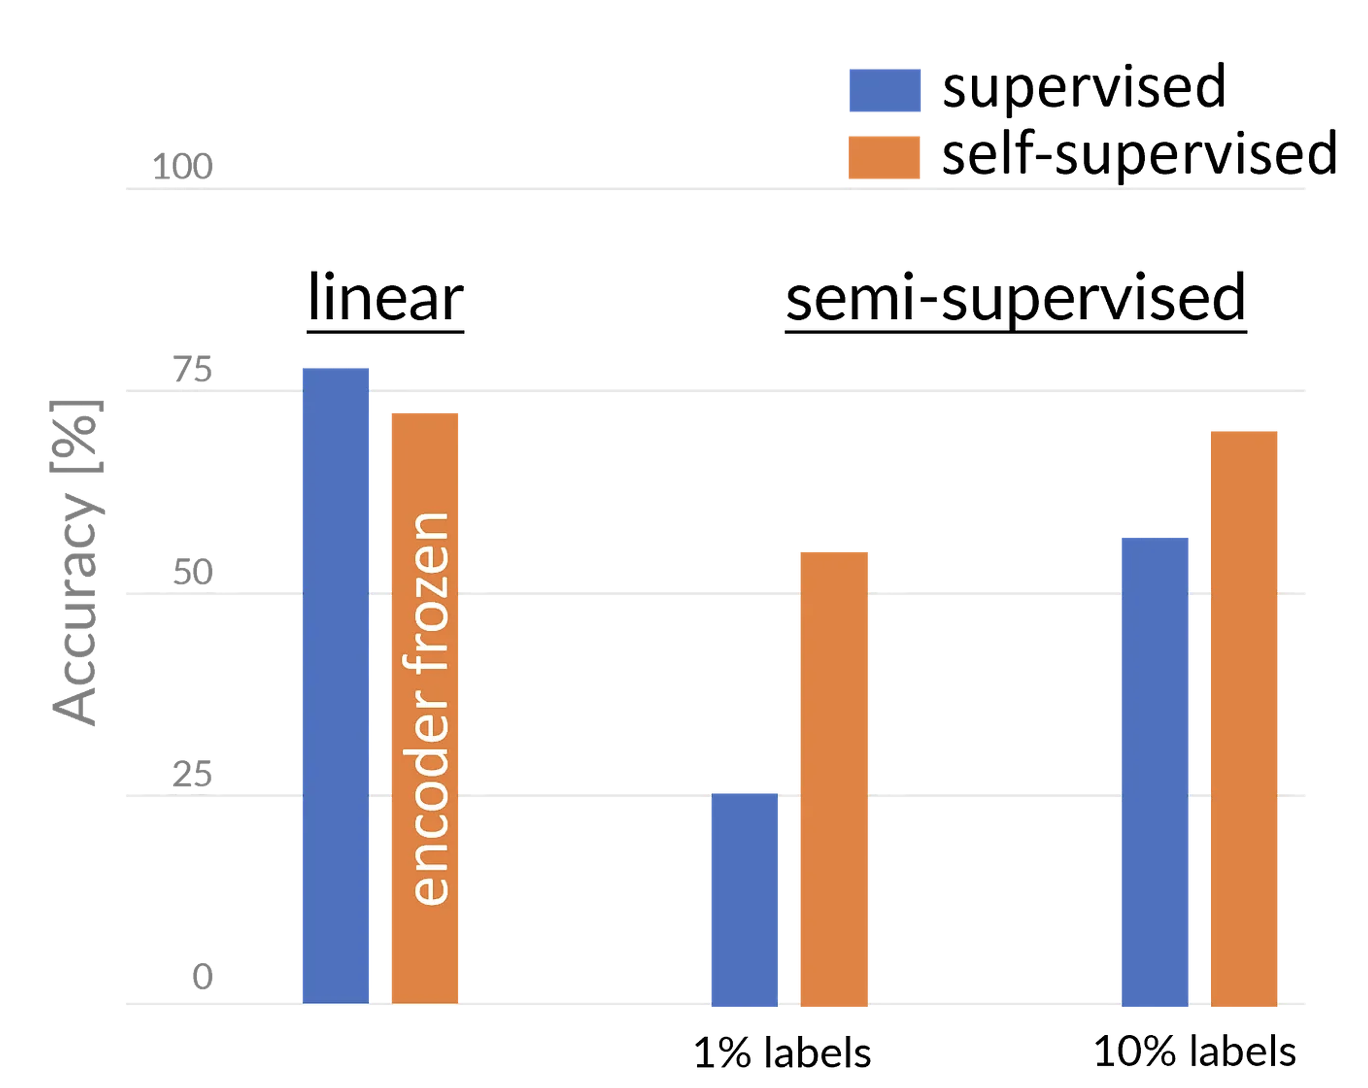
\includegraphics[scale=0.3]{../images/self_supervised_comparison.png}
     
\end{frame}


\begin{frame}
  \frametitle{fresh news}

  \begin{itemize}
    \item \href{https://ai.meta.com/blog/yann-lecun-ai-model-i-jepa/}{I-JEPA : The first AI model based on Yann LeCun's vision for more human-like AI}   
    \item \href{https://arxiv.org/abs/2303.03679}{MAST : Masked Augmentation Subspace Training for Generalizable Self-Supervised Priors}
  \end{itemize}
   
\end{frame}





\begin{frame}
  
  \frametitle{Montezuma's revenge - 10 years of tears?} 

    \begin{columns}
      \column{\dimexpr\paperwidth-10pt}

        source : \url{https://paperswithcode.com/sota/atari-games-on-atari-2600-montezumas-revenge}


        \begin{table}[]
        \begin{tabular}{|l|l|l|}
        \hline
        \textbf{year} & \textbf{name}                                       & \textbf{score} \\ \hline
        2013          & Playing Atari with Deep Reinforcement Learning      & 0              \\ \hline
        2015          & Deep Reinforcement Learning with Double Q-learning  & 0              \\ \hline
        2017          & Curiosity-driven Exploration by Self-supervised Prediction \footnote[1]{https://arxiv.org/abs/1705.05363} & 0       \\ \hline 
        2021          & MuZero                                              & 2500           \\ \hline
        2018          & Count-Based Exploration with Neural Density Models \footnote[2]{https://arxiv.org/abs/1703.01310}  & 3705           \\ \hline
        \textbf{2019} & \textbf{Exploration by Random Network Distillation} \footnote[3]{https://arxiv.org/abs/1810.12894}& \textbf{8152}  \\ \hline
        2021          & GoExplore$^*$ \footnote[4]{https://arxiv.org/abs/2004.12919}                         & 43 000         \\ \hline
        \end{tabular}
        \end{table}

        {\bf * requires environment state saving/loading}

    \end{columns}


\end{frame}





\begin{frame}
  
  \frametitle{sample efficiency}

  \begin{itemize}
    \item RND \footnote{\href{https://arxiv.org/pdf/1810.12894.pdf}{Burda et al. 2018}} $4.5*10^9$ samples, score 8152 on MR
    \item Never give up \footnote{\href{https://arxiv.org/pdf/2002.06038.pdf}{Badia et al. 2020}} $3.5*10^{10}$ samples, score 10 000 on MR
    \item SND $1.28*10^8$ samples with score 25 000 
  \end{itemize}

  NGU on my machine means {\bf 740 days} !!!
\end{frame}


\begin{frame}{\bf random network distillation}
  
  \begin{columns}

    \begin{column}{0.5\textwidth}
      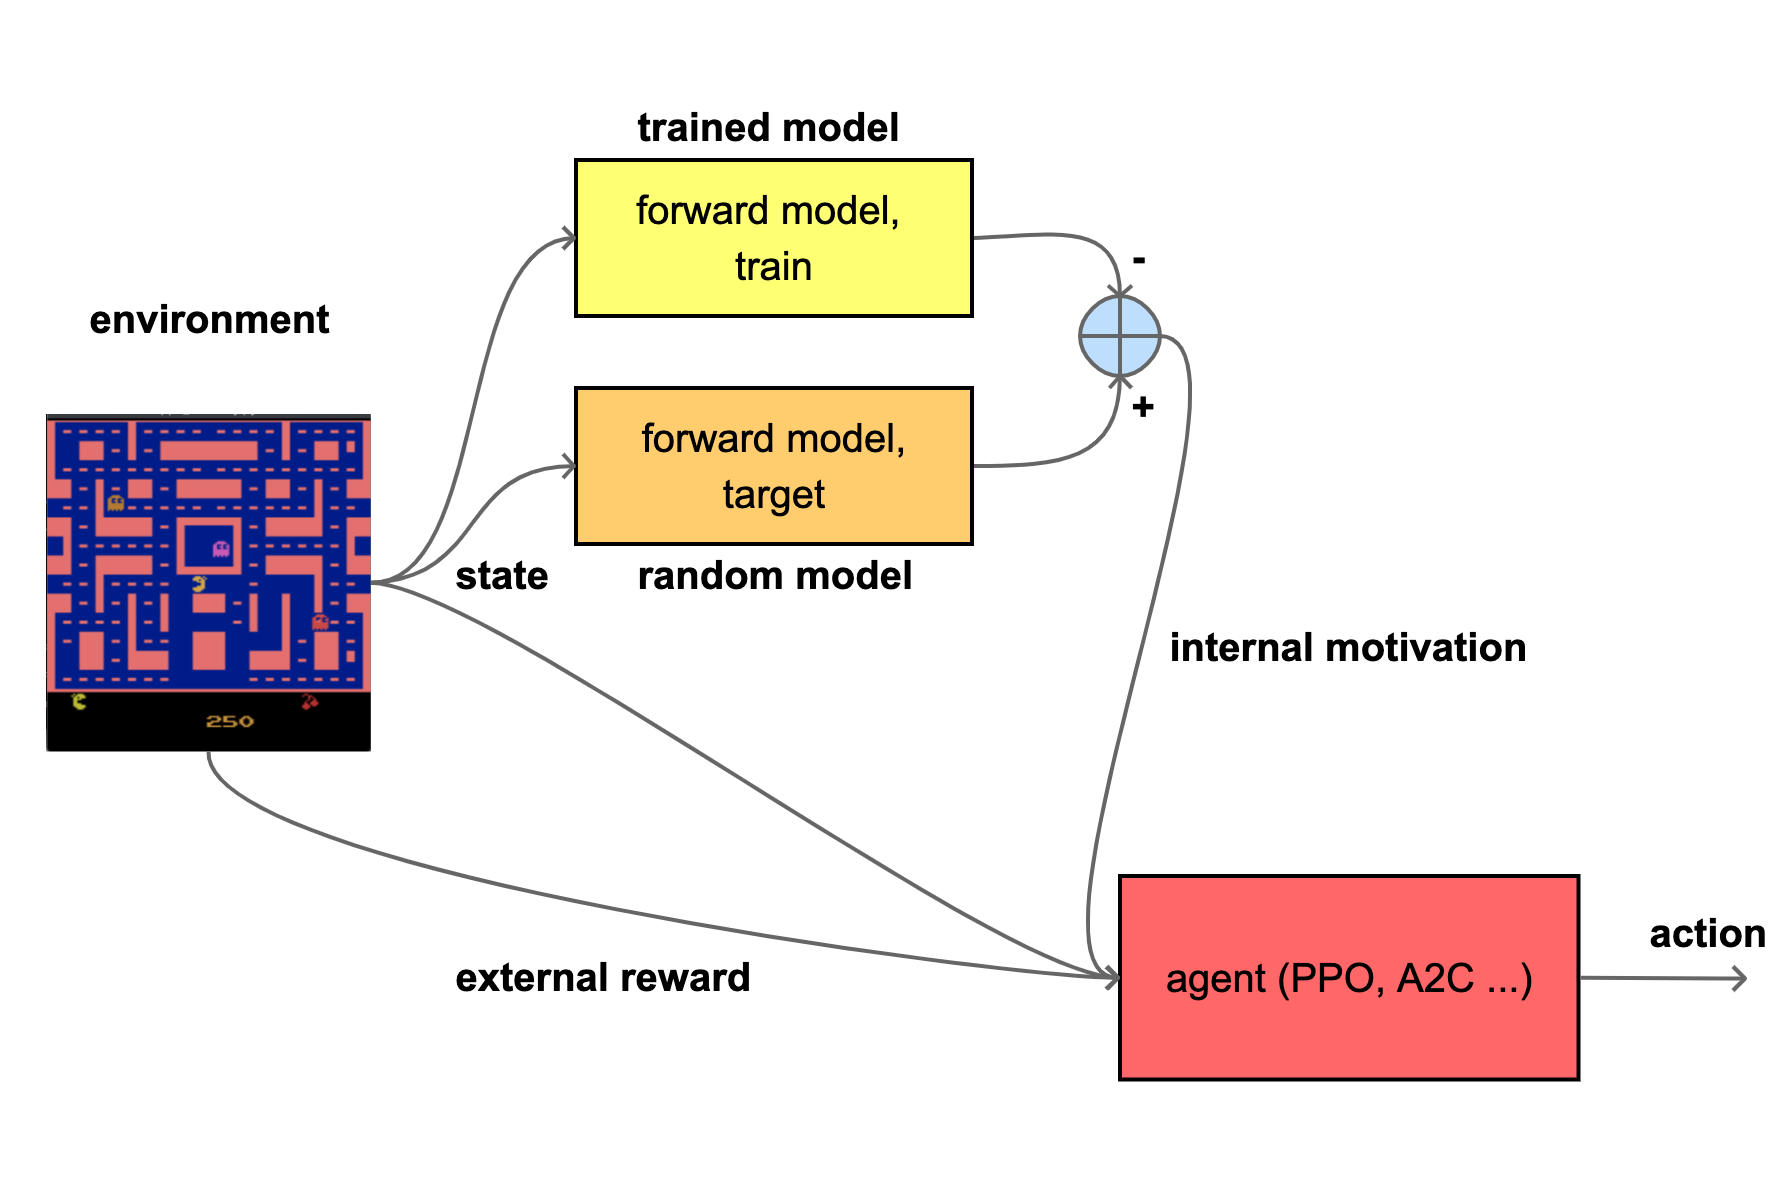
\includegraphics[scale=0.1]{../diagrams/rnd/rnd.png}
    \end{column}

    \begin{column}{0.5\textwidth}
      \begin{itemize}
        \item neural network works as {\bf novelty detector}
        \item model learns to imitate random (target) model
        \item {\bf less visited states produce bigger motivation signal}
        \item orthogonal weights initialisation ($g=2^{0.5}$) for strong signal
        \item lot of fully connected layers {\bf to avoid generalisation}
      \end{itemize}
    \end{column}


  \end{columns}
  
\end{frame}
  


\begin{frame}
  \frametitle{Exploration by self supervised-exploitation}
  Matej Pecháč, Michal Chovanec, Igor Farkaš

  \centering
  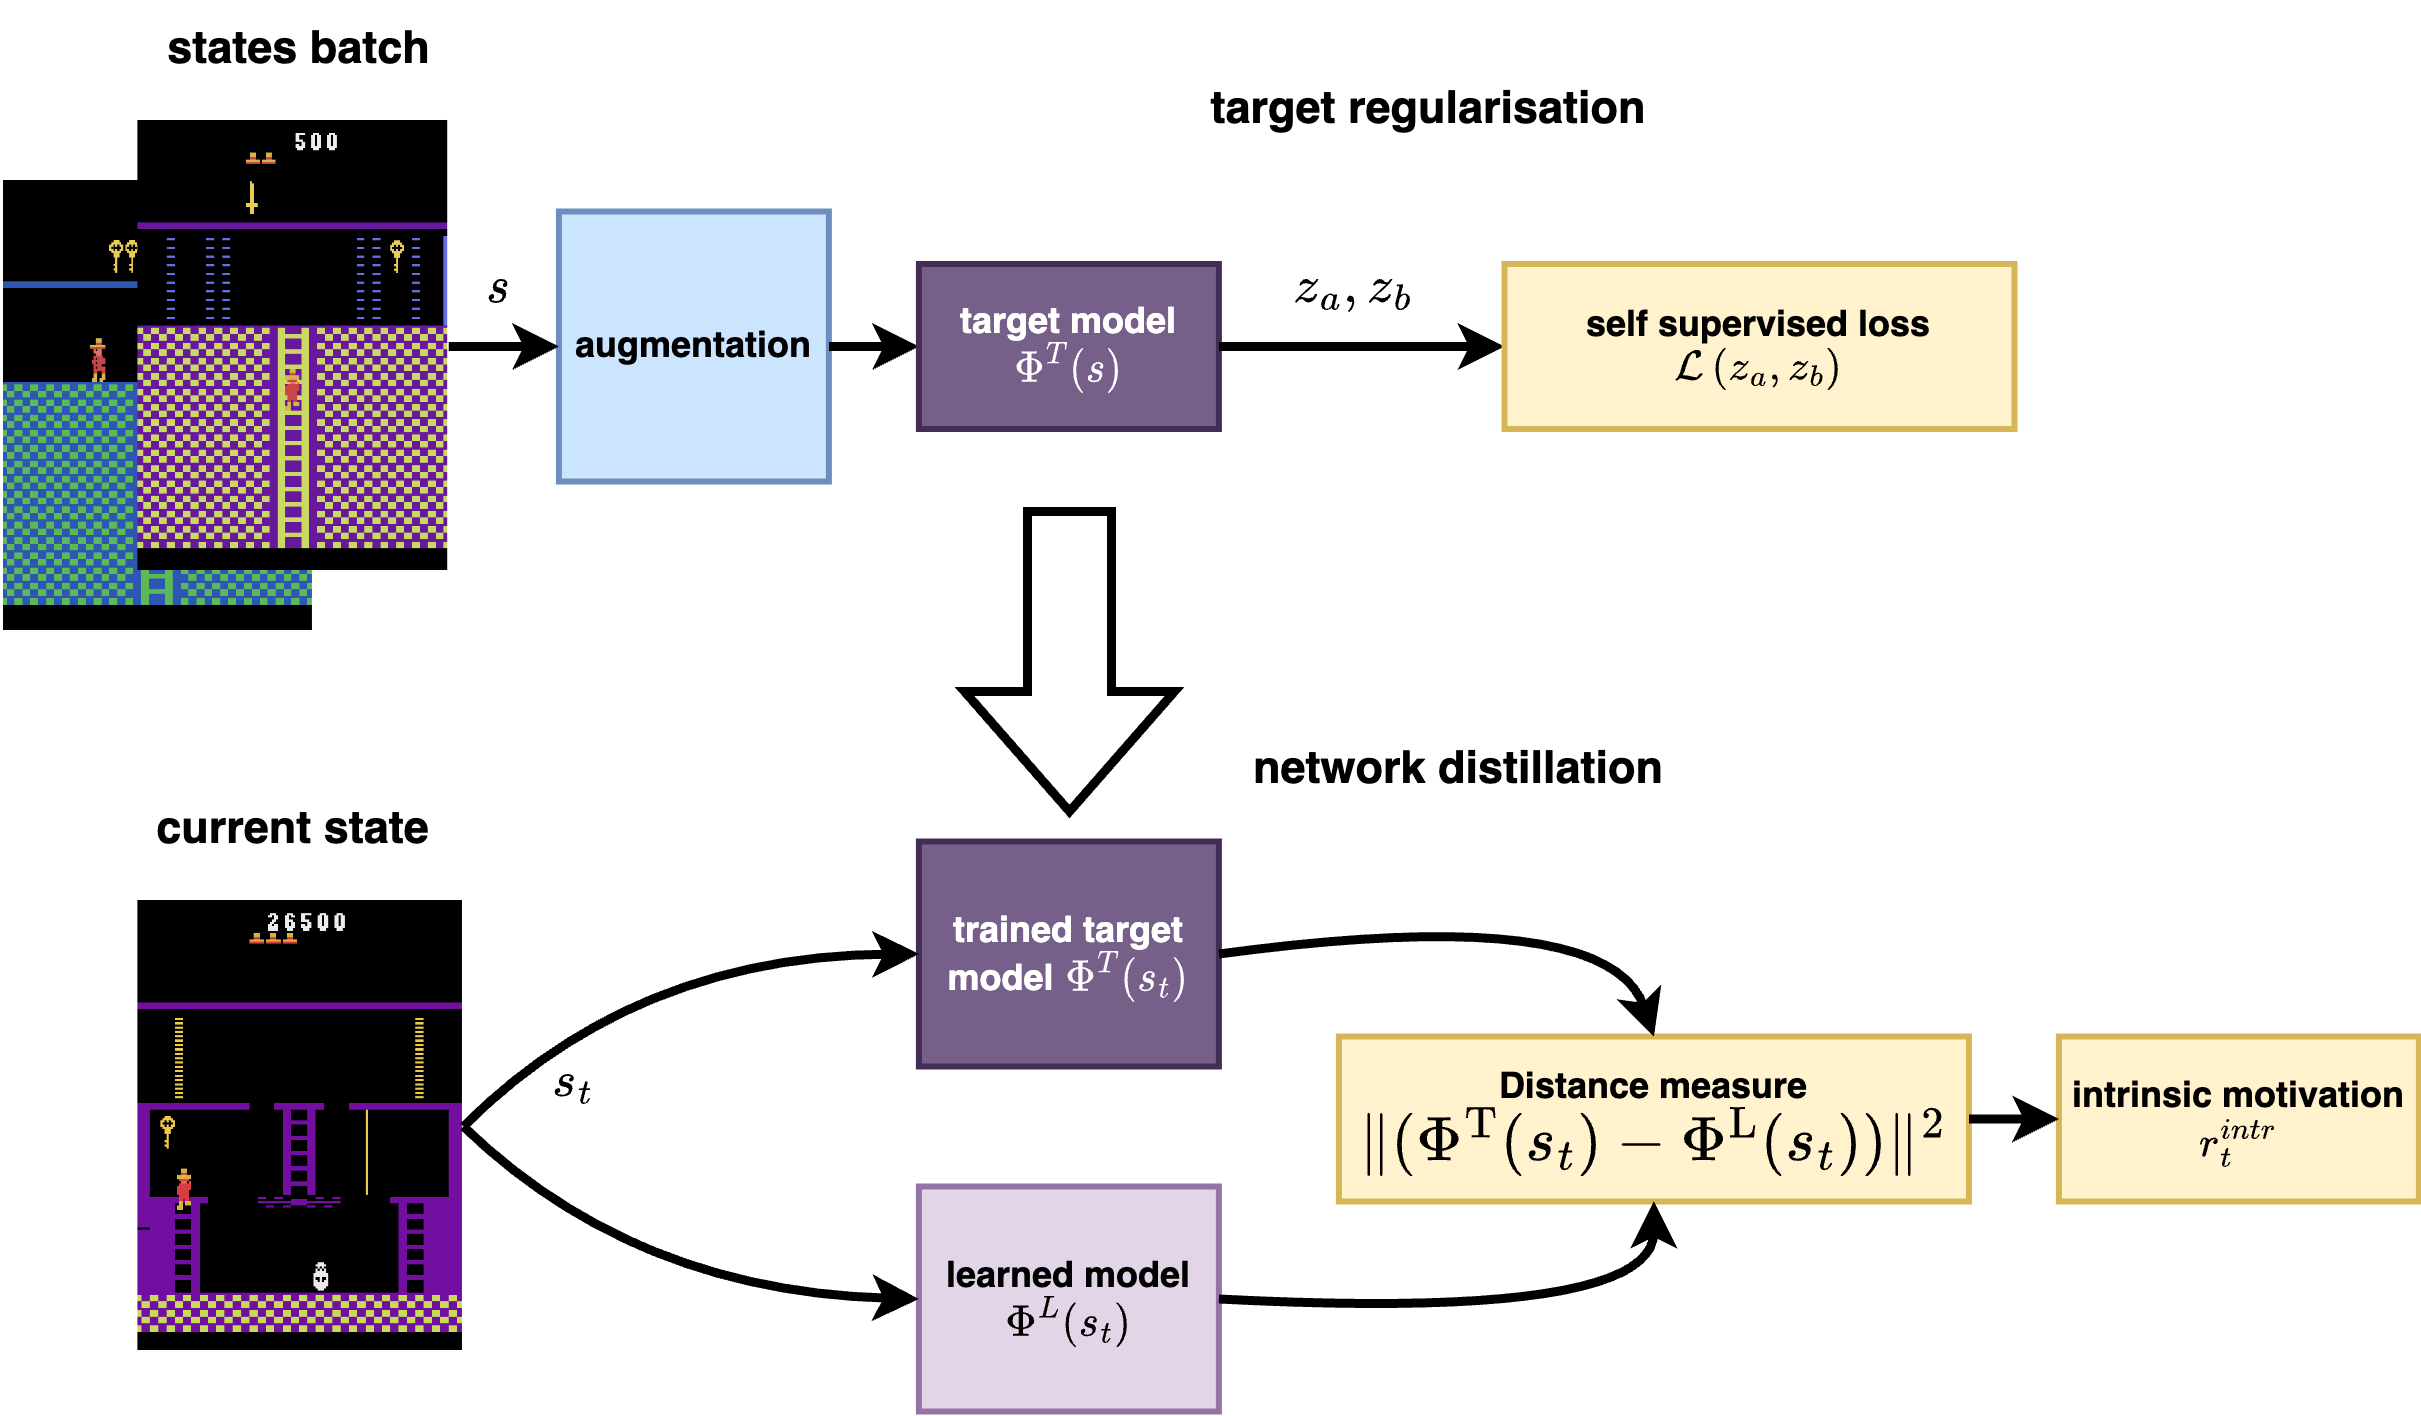
\includegraphics[scale=0.5]{../diagrams/cnd/cnd-cnd.png}

\end{frame}



\begin{frame}
  \frametitle{Exploration by self supervised-exploitation}
  \begin{itemize}
    \item we extended existing idea of Random Network Distillation
    \item {\color{red} 1 : } for target model, self supervised training is used
    \item {\color{red} 2 : } augmented states are used to train target model
    \item {\color{red} 3 : } target model is used as distillation source
    \item {\color{red} 4 : } distillation error is used for intrinsic motivation
  \end{itemize} 

  \vskip 0pt plus 1filll 
    \centering
    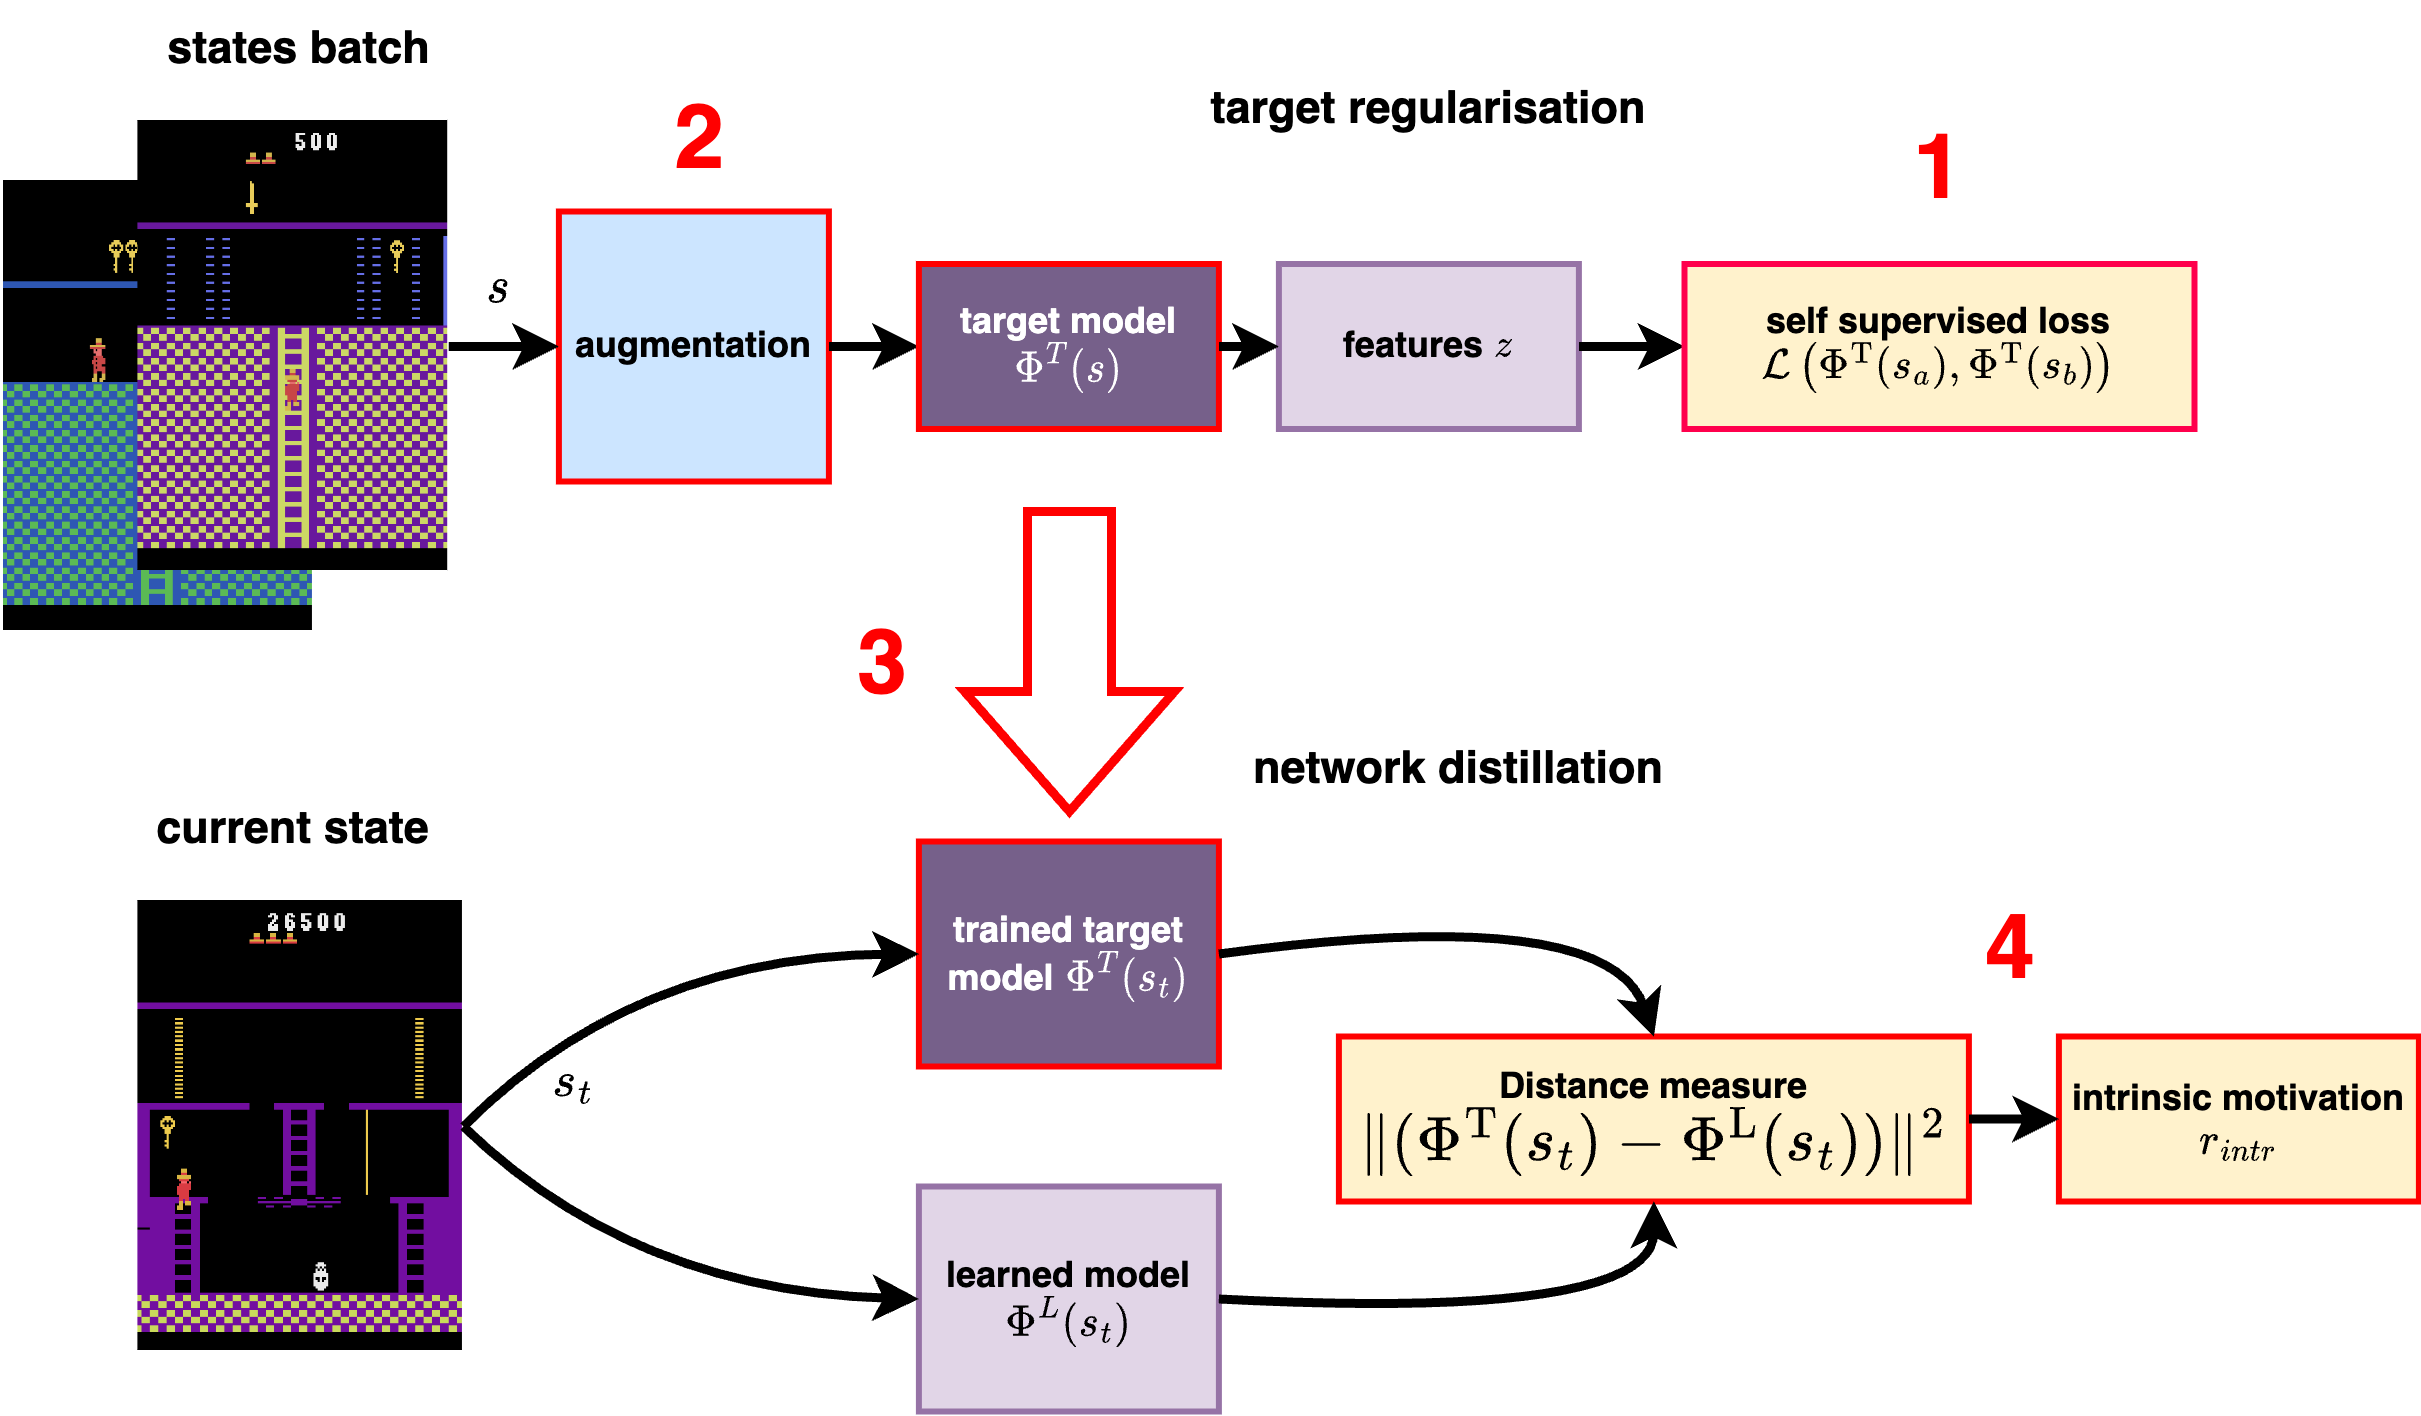
\includegraphics[scale=0.4]{../diagrams/cnd/cnd-cnd-4.png}

\end{frame}


\begin{frame}
  \frametitle{Trained features}

  \begin{itemize}
    \item t-SNE features projection for random and trained models
    \item color represents different rooms in Atari Montezuma's Revenge 
    \item self supervised features provides much bigger variance
    \item preventing agent to stuck
  \end{itemize} 
  
  \vskip 0pt plus 1filll 
  \begin{columns}
  
    \begin{column}{0.5\textwidth}
      random features
      \bigskip
      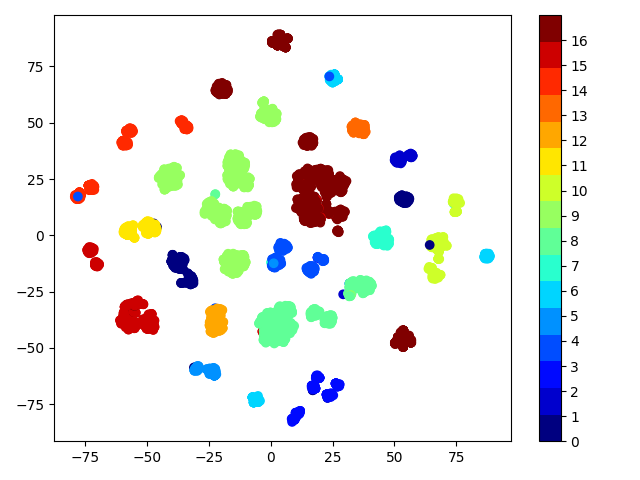
\includegraphics[scale=0.35]{../images/cnd_random.png}
    \end{column}

    \begin{column}{0.5\textwidth}
      self supervised trained features
      \bigskip
      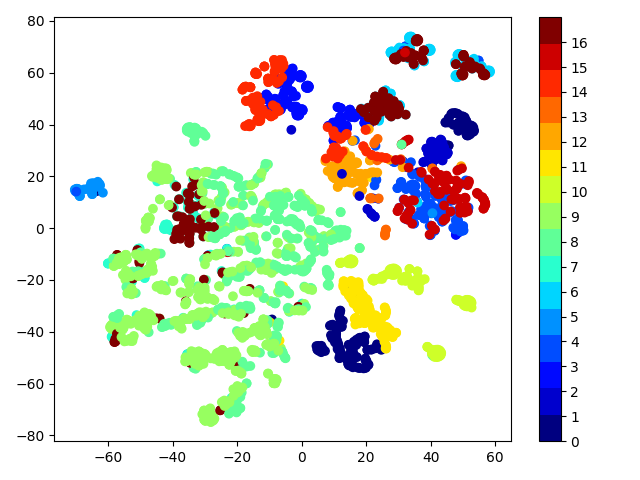
\includegraphics[scale=0.35]{../images/cnd_trained.png}
    \end{column}
  
  \end{columns}
  
\end{frame}


\begin{frame}
  \frametitle{Exploration signal}
  
  \begin{itemize}
    \item Random Network Distillation signal decrease over time
    \item our method provides more informative signal
  \end{itemize} 
  
  \vskip 0pt plus 1filll 
  {\Large Random Network Distillation} \\
  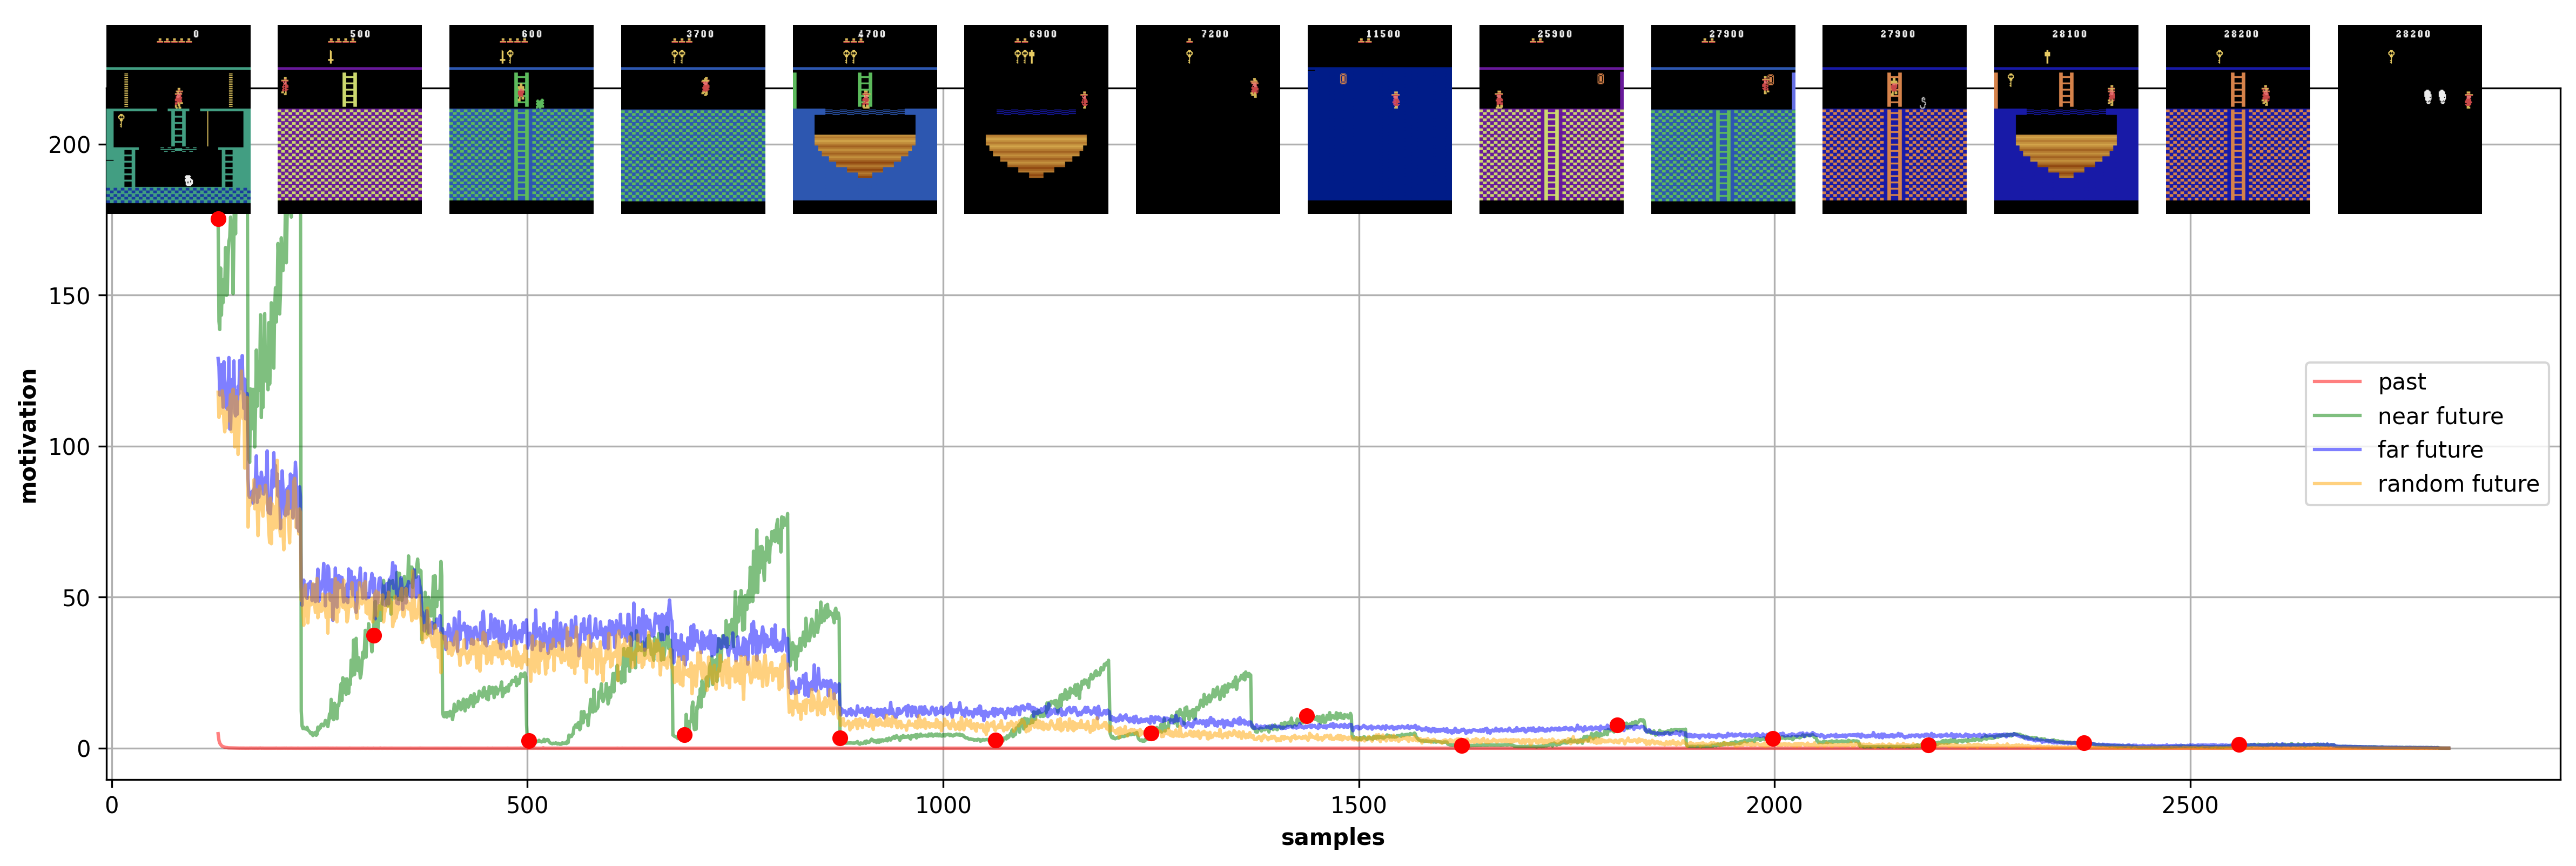
\includegraphics[scale=0.2]{../results/novelty_detection/rnd_result_summary.png}
  \\
  {\Large our method} \\
  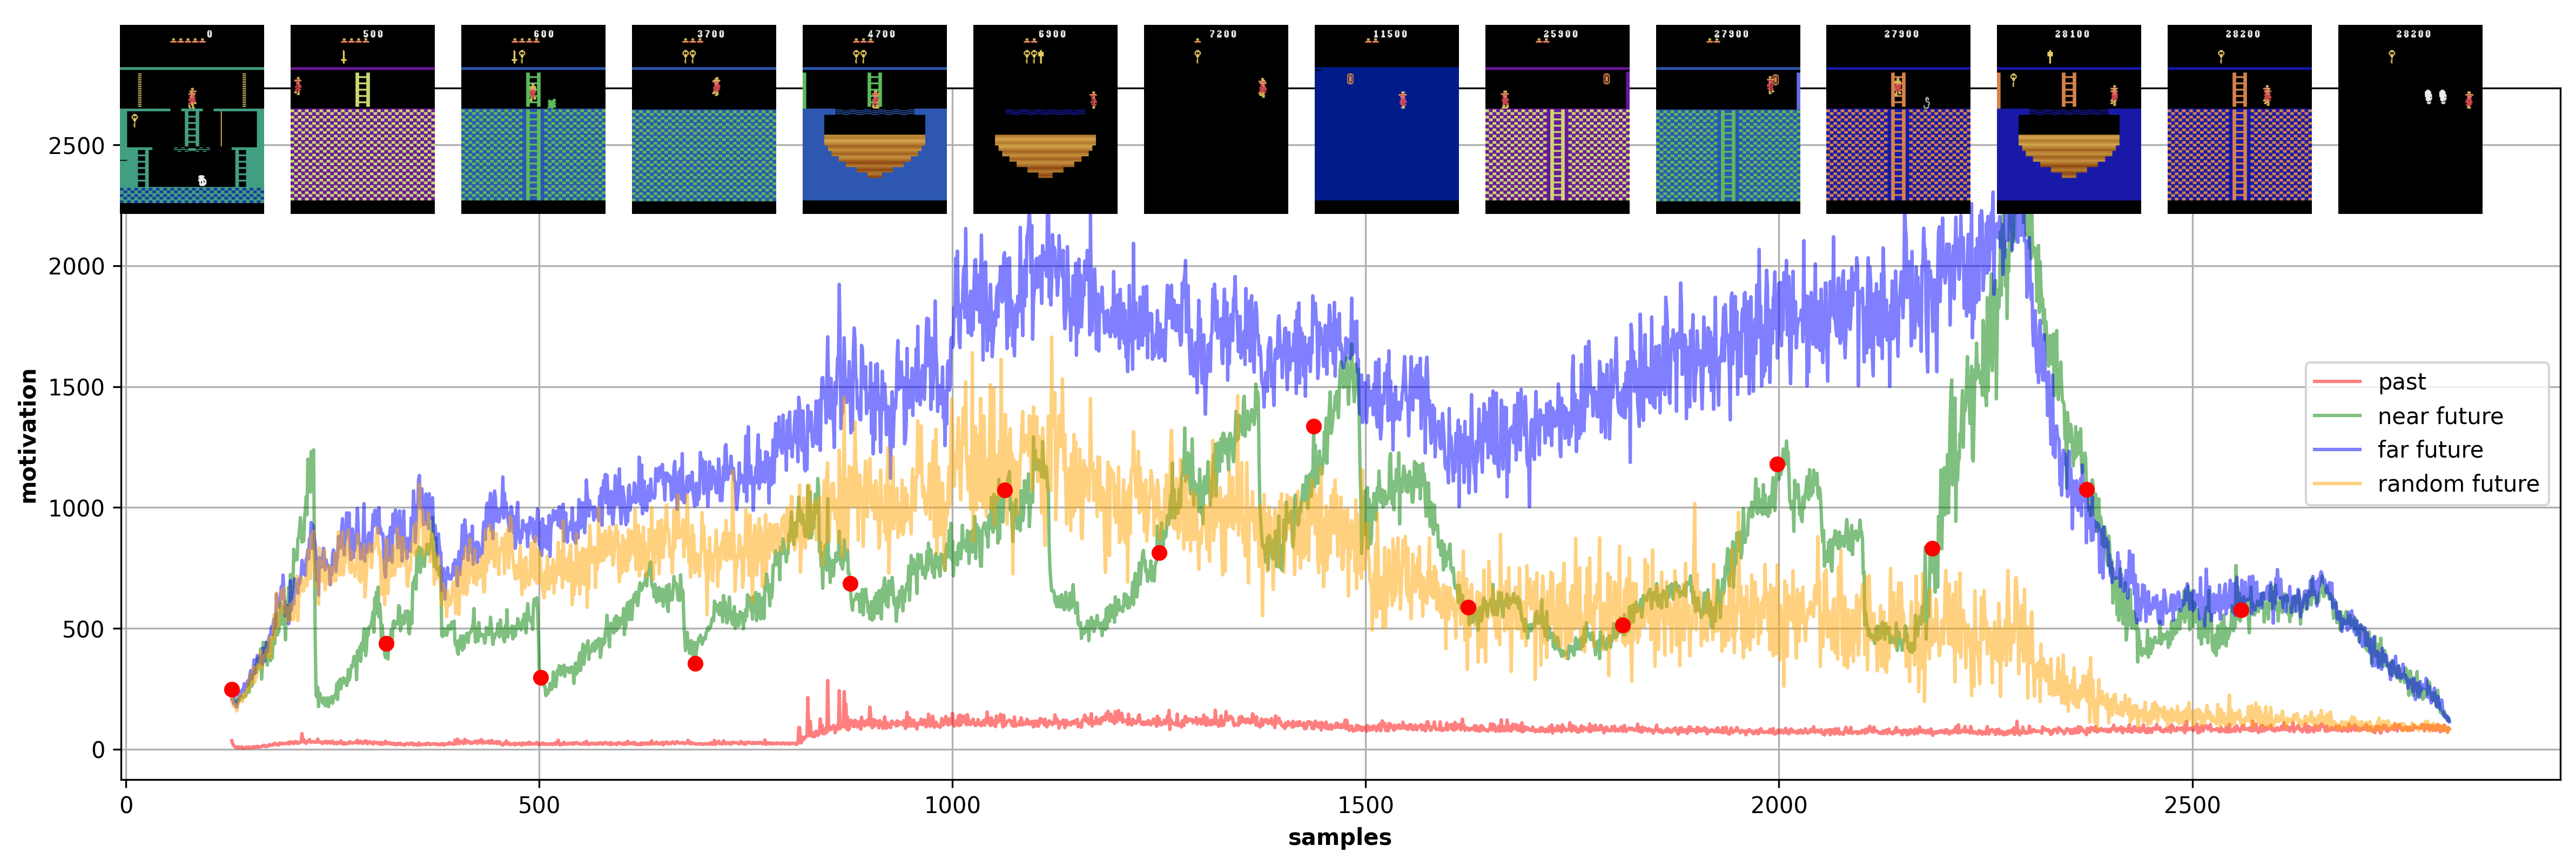
\includegraphics[scale=0.2]{../results/novelty_detection/cnd_vicreg_result_summary.png}

\end{frame}


\begin{frame}
  \frametitle{Results}

  \begin{itemize}
    \item Montezuma's Revenge, with score {\color{red}25 000+}
    \item Private Eye, with score {\color{red}12 000+}
    \item Venture, Gravitar 
    \item 128M samples total - only single GPU needed
  \end{itemize} 
  
  
  \begin{columns}
  
    \begin{column}{0.5\textwidth}
      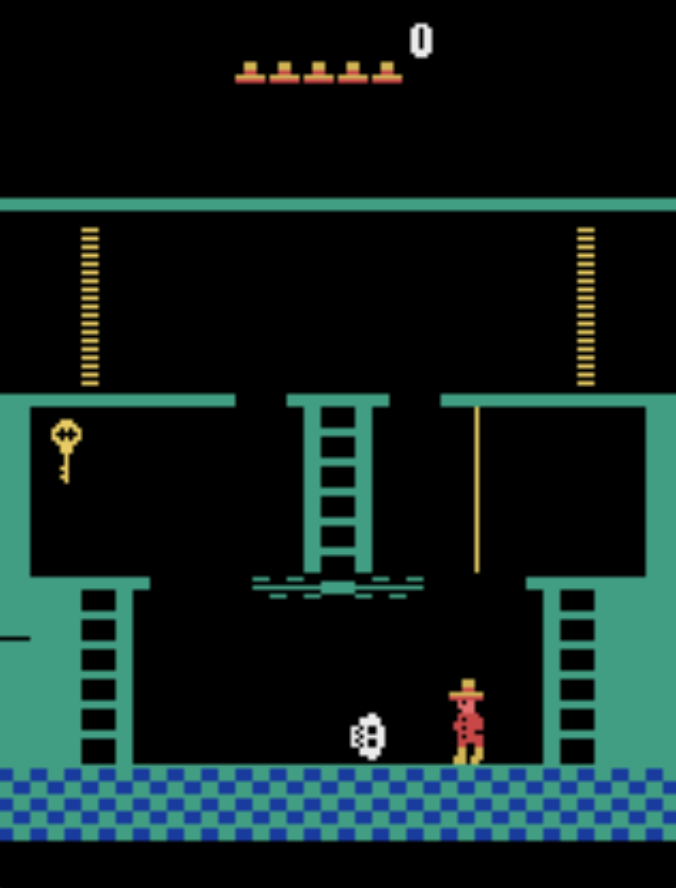
\includegraphics[scale=0.32]{../images/montezuma.png}
    \end{column}

    \begin{column}{0.5\textwidth}
      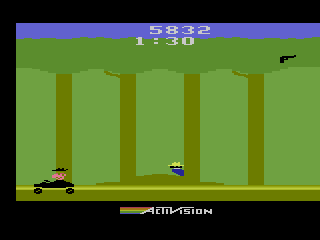
\includegraphics[scale=0.4]{../images/privateeye.png}
    \end{column}
  
  \end{columns}

\end{frame}






\begin{frame}
  \frametitle{Results}
  
  {\Large solved Procgen hard exploration seeds} \\
  environments : Caveflyer, Climber, Coinrun, Jumper
  
  \begin{columns}
  
    \begin{column}{0.6\textwidth}
      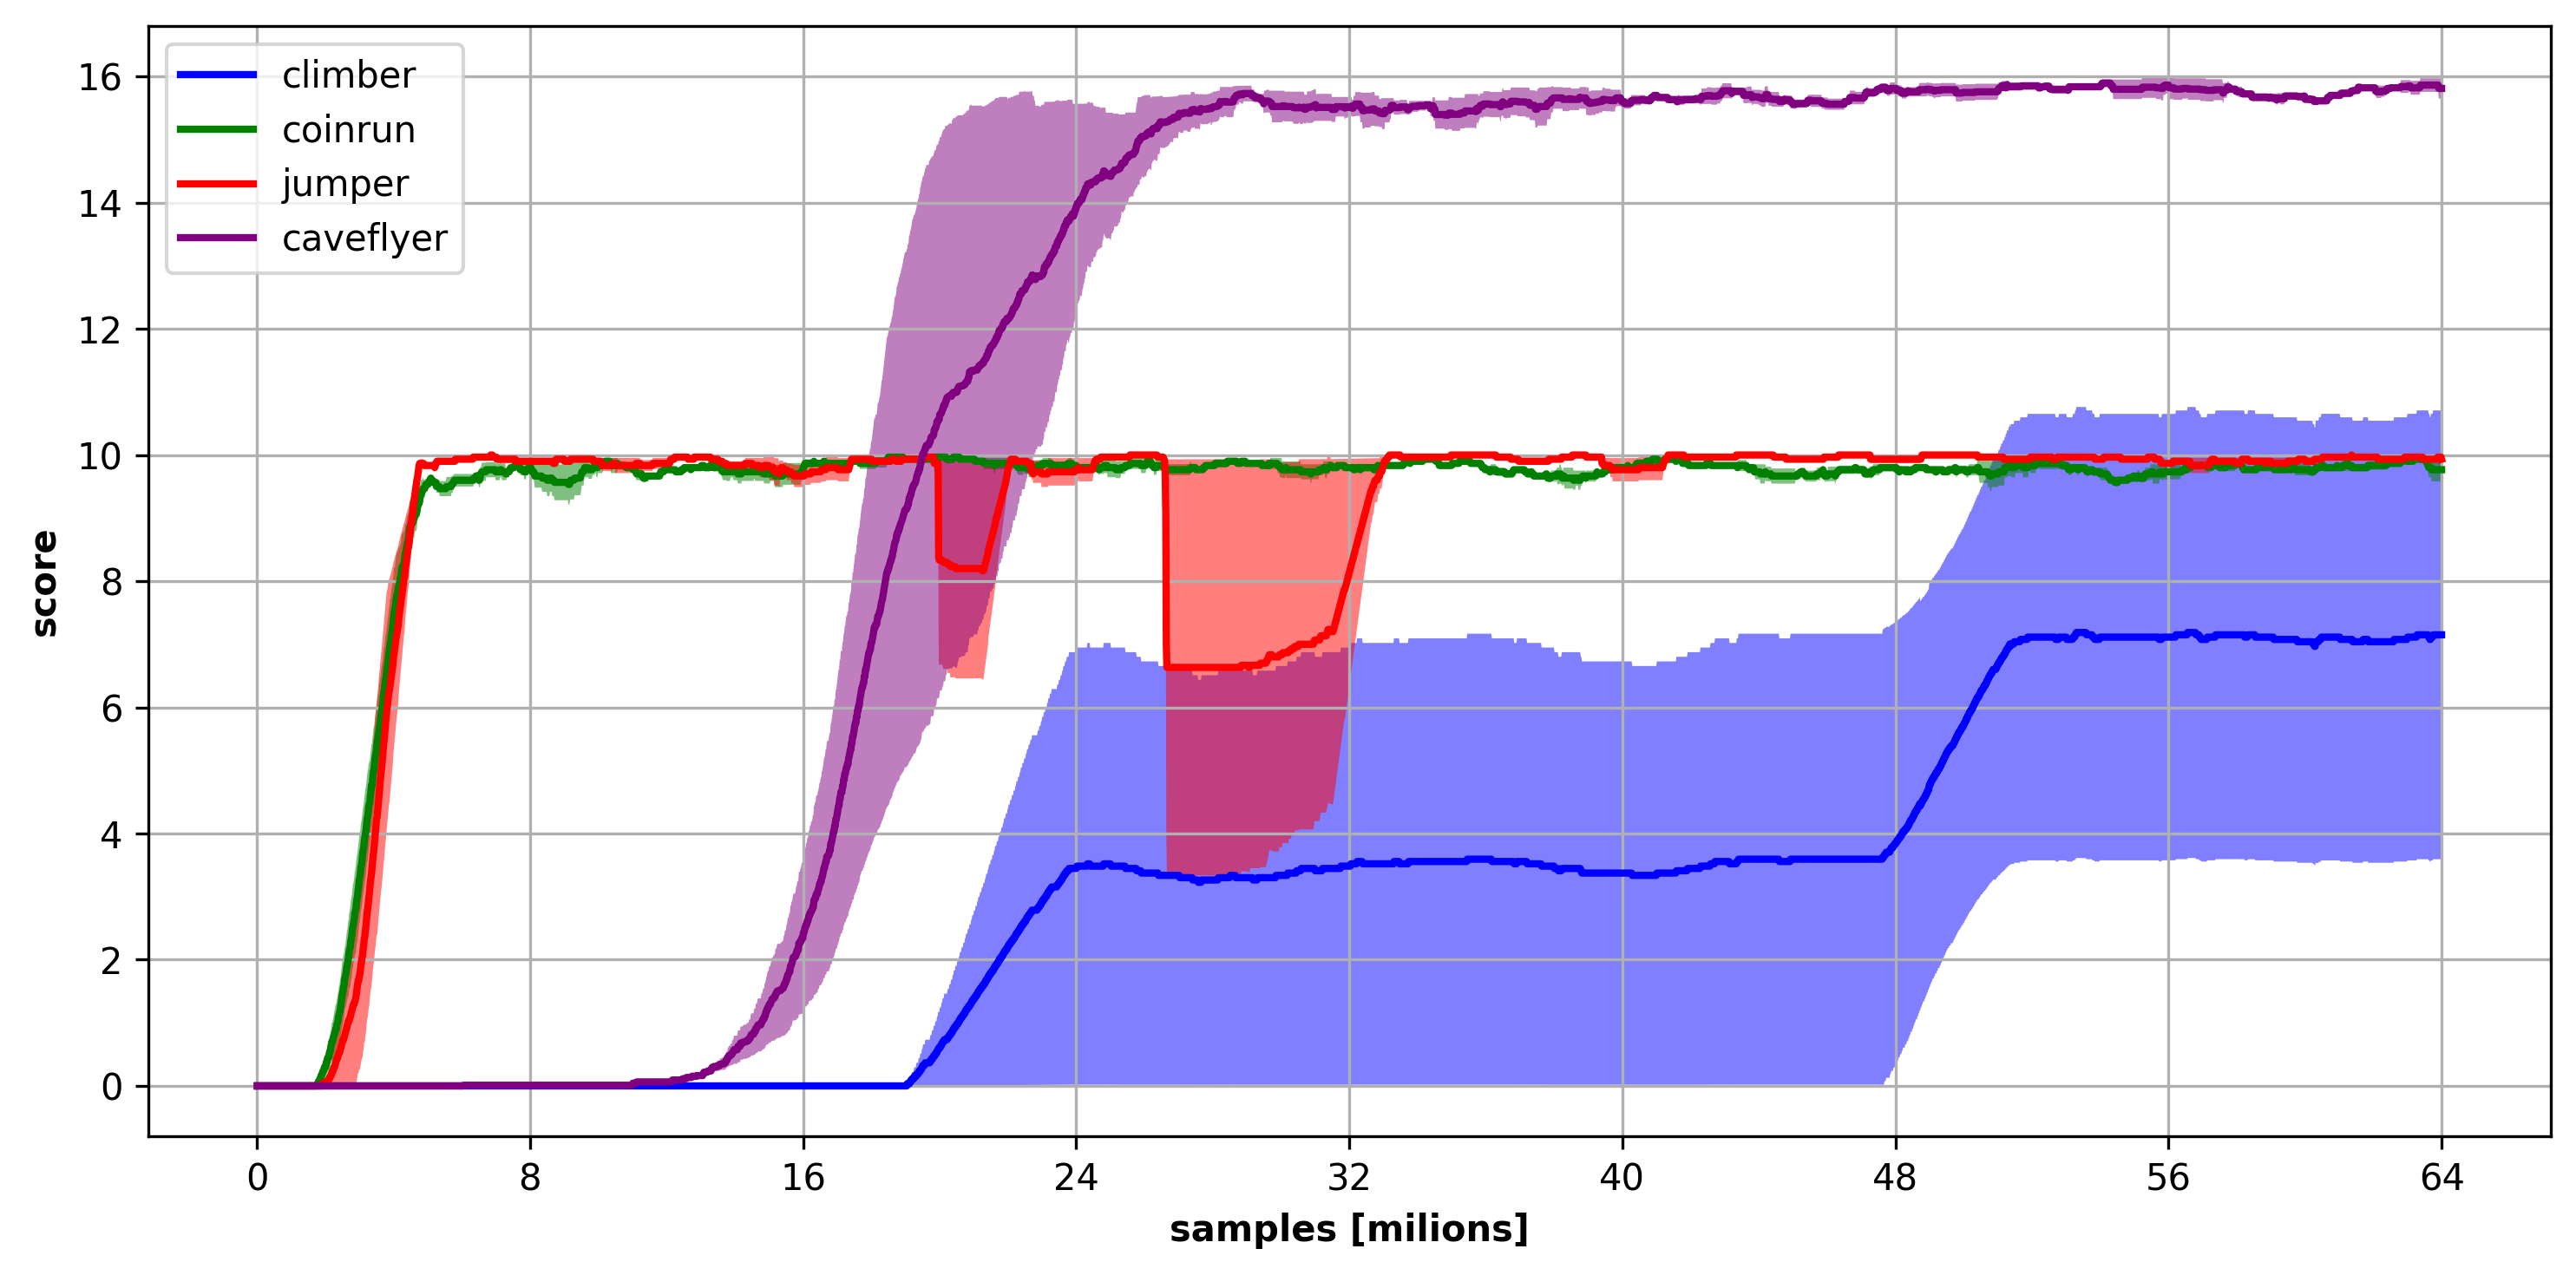
\includegraphics[scale=0.25]{../results/summary/procgen_all_score.png}
    \end{column}

    \begin{column}{0.4\textwidth}
      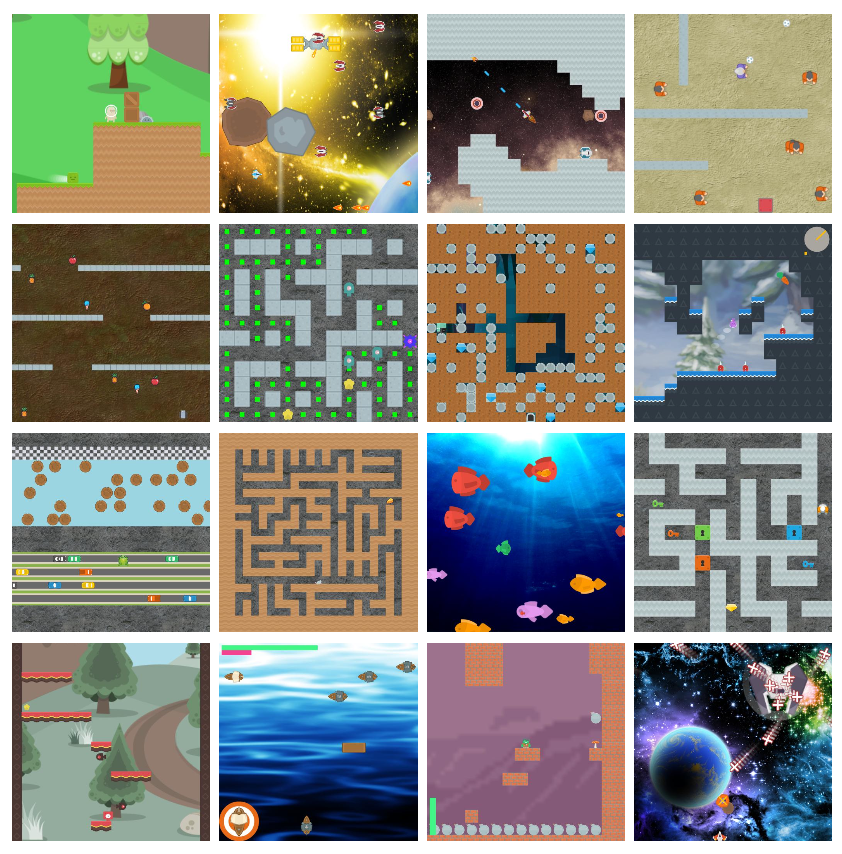
\includegraphics[scale=0.25]{../images/procgen.png}
    \end{column}
  
  \end{columns}

\end{frame}




























\begin{frame}
  
  \frametitle{misleading papers - Curiosity-driven Exploration by Self-supervised Prediction \footnote{\href{https://arxiv.org/abs/1705.05363}{Pathak et al. 2017}}}
  
  \begin{itemize}
    \item not working on REAL hard exploration problems
    \item Super Mario is special case - moving forward is close to optimal policy
    \item inverse ICM model - why they didn't shown accuracy (my results arround only 40\% !!!)
    \item how predicted state looks ?
  \end{itemize}

  \centering
  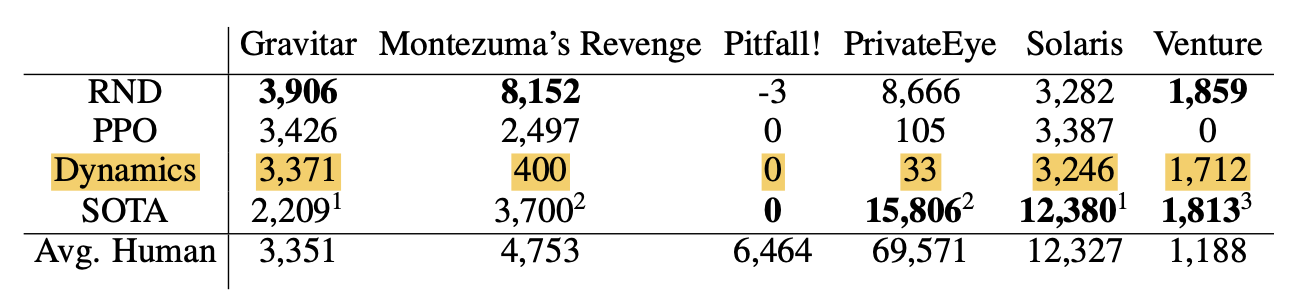
\includegraphics[scale=0.25]{../papers_captions/icm_a.png}

\end{frame}



\begin{frame}
  
  \frametitle{misleading papers - Never give up \footnote{\href{https://arxiv.org/pdf/2002.06038.pdf}{Badia et al. 2020}}}
  nice looking score, but on cost of $3.5*10^{10}$ samples !!!
  
  \centering
  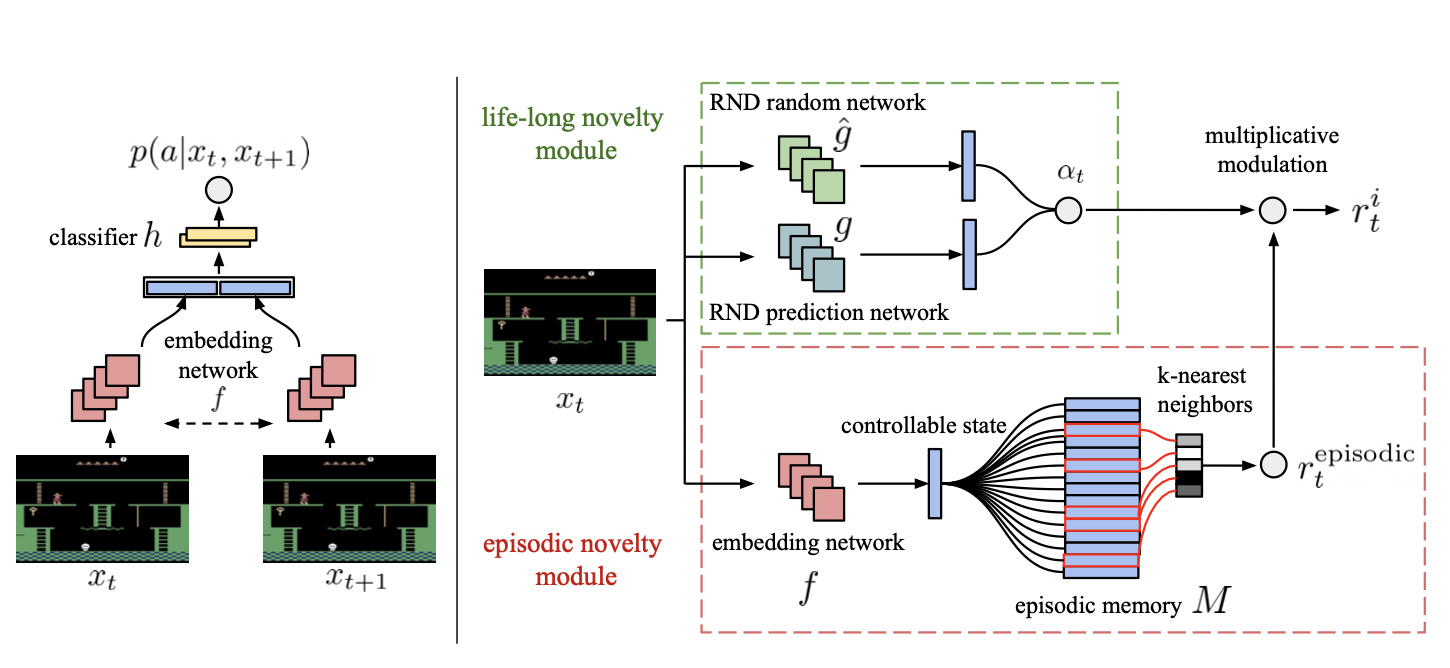
\includegraphics[scale=0.25]{../papers_captions/ngu_block.png}

  \centering
  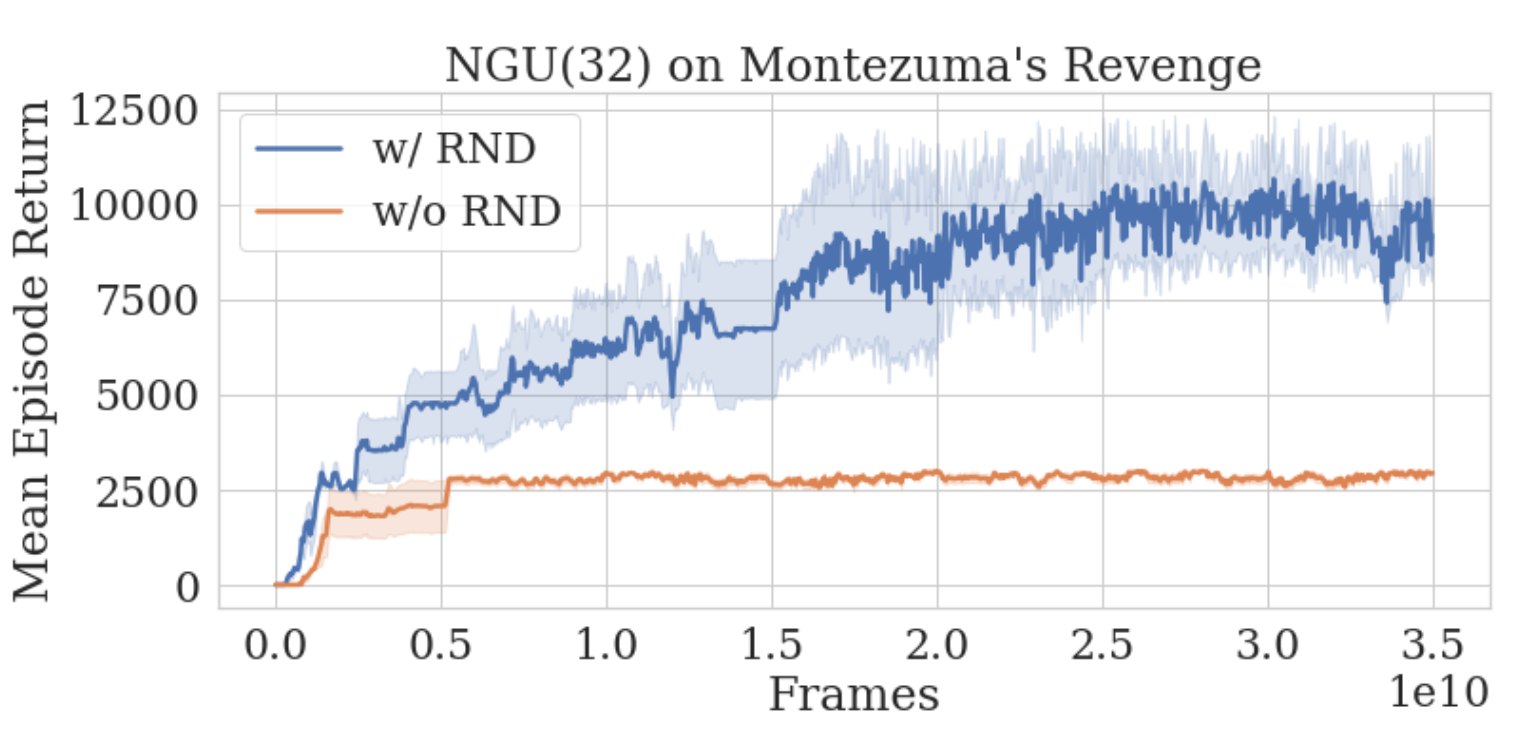
\includegraphics[scale=0.25]{../papers_captions/ngu_result.png}

\end{frame}



\begin{frame}
  
  \frametitle{other misleadings}

  \centering
  {\bf avoiding comparing with SOTA or common benchmarks results} :
  Episodic Curiosity Through Reachability, Savinov, 2019 
  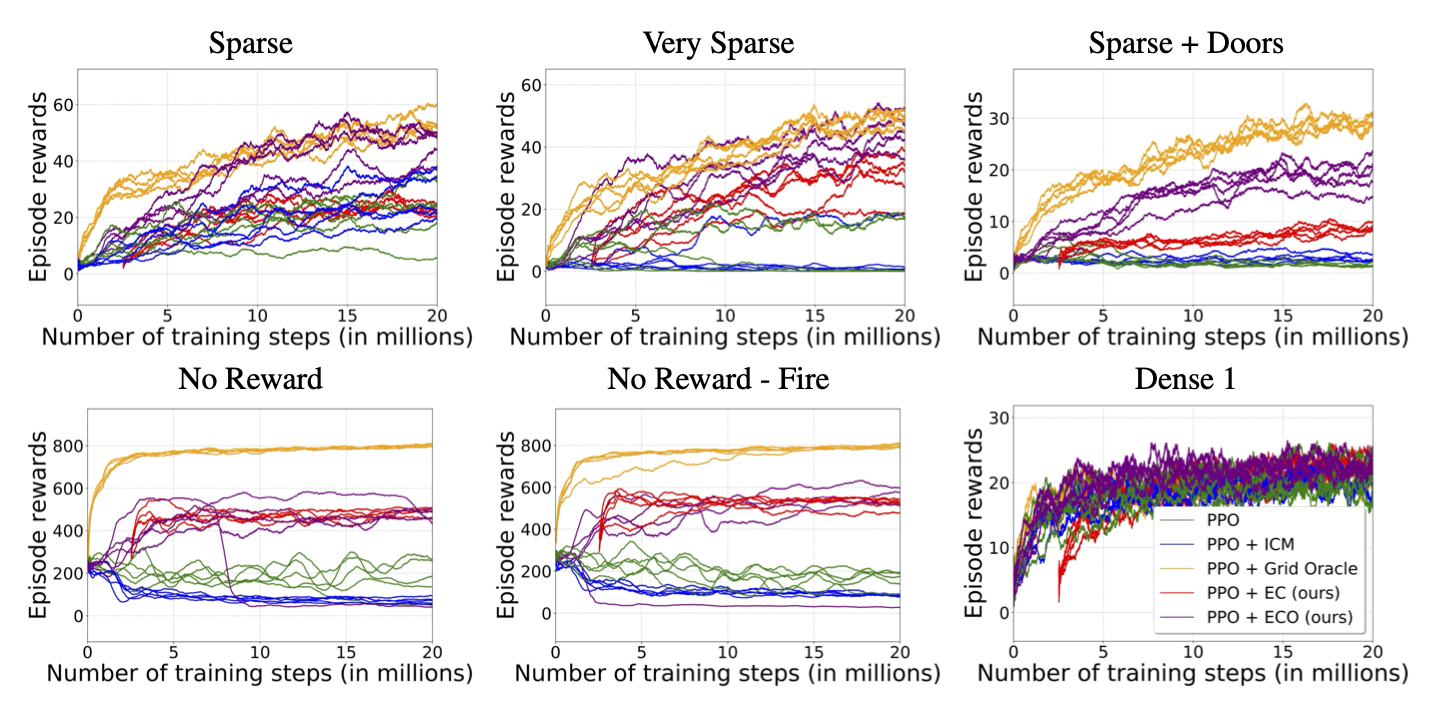
\includegraphics[scale=0.25]{../papers_captions/ecr.png}
  \bigskip

  many other :

  \begin{itemize}
    \item simple gridworld or toy environment experiments
    \item providing key prior information (e.g. possition)
    \item selecting only "good" results
  \end{itemize}

\end{frame}




\begin{frame}
  
  \frametitle{Q\&A}

  \begin{columns}

    \begin{column}{0.5\textwidth}
      \centering{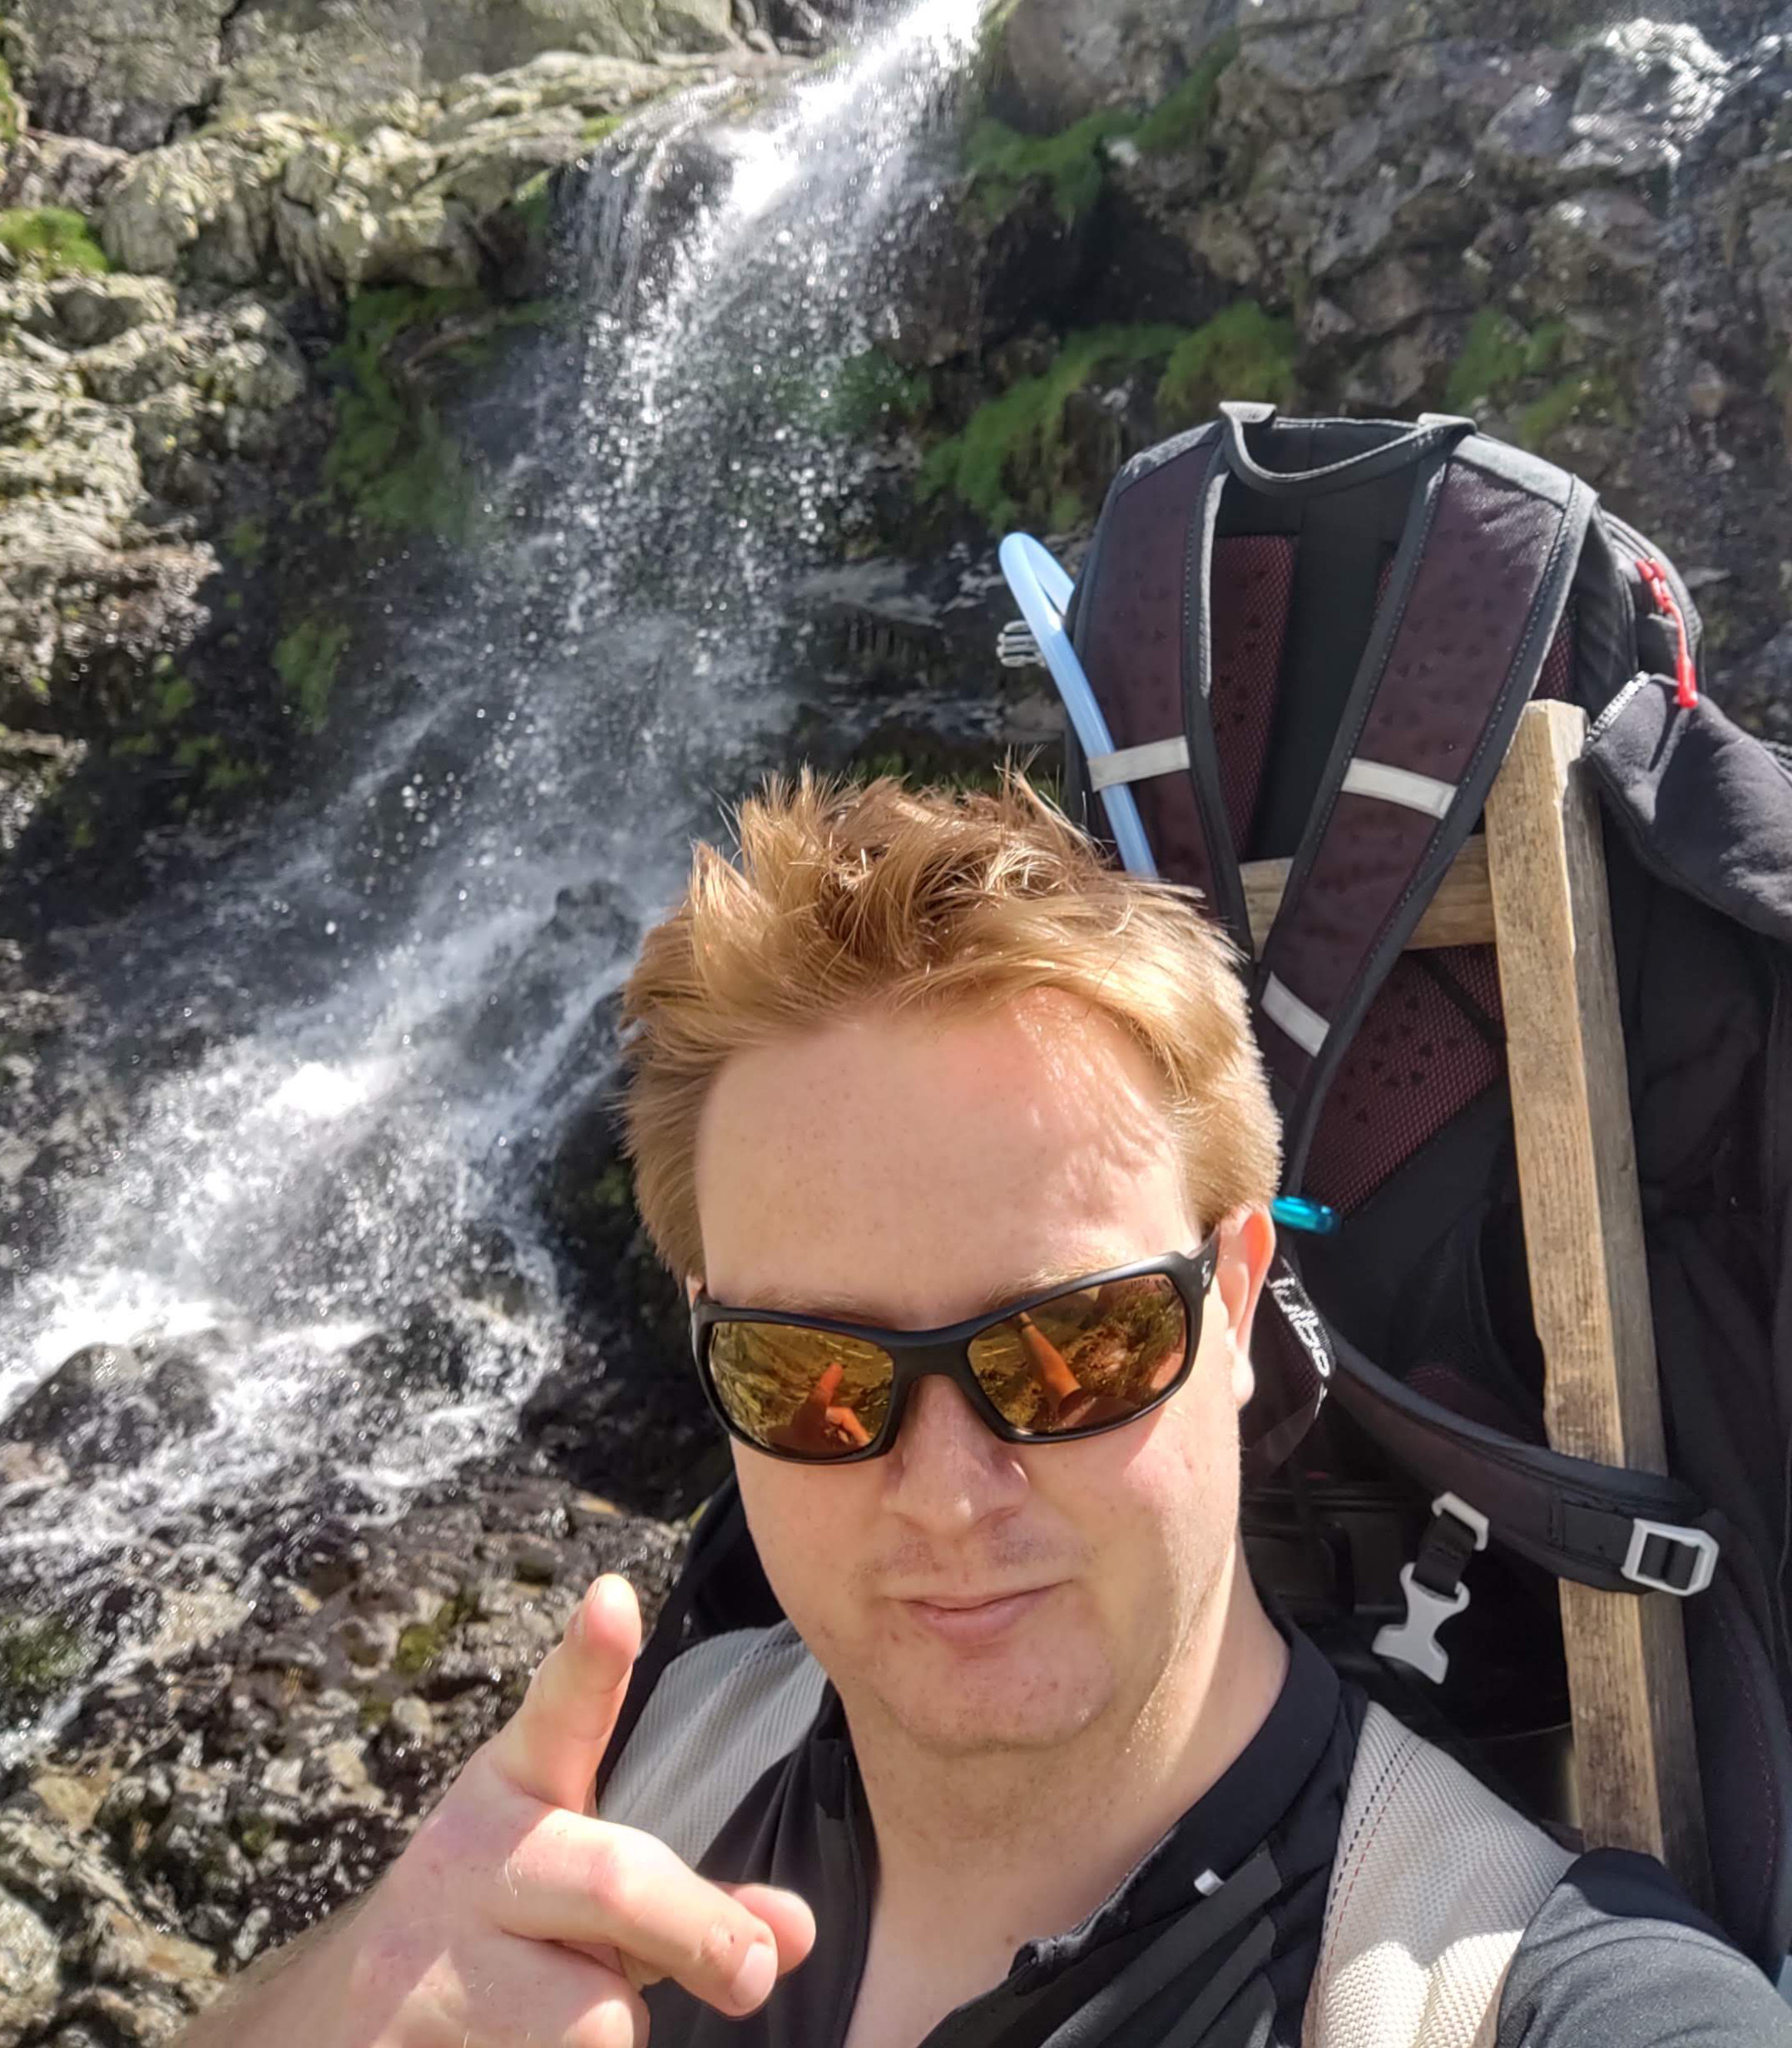
\includegraphics[scale=0.08]{../images/me.jpg}}
    \end{column}

    \begin{column}{0.5\textwidth}
      \begin{itemize}
        \item \url{https://github.com/michalnand/}
        \item \url{michal.nand@gmail.com}
      \end{itemize}
    \end{column}

  \end{columns}

    
\end{frame}



\end{document}